\PassOptionsToPackage{unicode=true}{hyperref}
\documentclass[envcountsect,aspectratio=169]{beamer}
%\documentclass[envcountsect,mathserif,aspectratio=43]{beamer}
\usepackage{etex}


%\documentclass[envcountsect,mathserif]{beamer}
\usefonttheme[onlymath]{serif}
\usepackage[utf8x]{inputenc}
\usepackage[brazilian]{babel}
\usepackage{amsthm}
\usepackage{amssymb,mathtools}
\usepackage{amsmath}
\usepackage{graphicx}
\usepackage{wrapfig}
\usepackage{color}
\usepackage{multicol}
\usepackage{syntonly}
\usepackage{pgf,tikz}
\usepackage{enumerate}
%\usepackage{hyperref}
\usetikzlibrary{arrows.meta, bending, decorations.markings}

%\usepackage[colorlinks=true,allcolors=blue]{hyperref}
\usepackage{hyperref}
\usepackage{bookmark}
\pdfstringdefDisableCommands{\let\backslash\textbackslash}
\hypersetup{psdextra}

\usepackage[labelformat=empty]{caption}


\usetikzlibrary{arrows}

%\usepackage{tabularx}
%\usepackage{booktabs}
%\usepackage{colortbl}
\usetikzlibrary{calc}


%\syntaxonly
%\includeonly{bibliografia,espacos-normados,operadores-lineares,hanh-banach,grafico-fechado, top-fracas}%
%\usebackgroundtemplate{\includegraphics{calculus2.eps}}


%\definecolor{estrutura}{RGB}{110, 139, 61}
%\definecolor{darkolivegreen}{RGB}{85, 107, 47}
%\definecolor{palegreen}{RGB}{152, 251, 152}
%\definecolor{DarkSeaGreen}{RGB}{143, 188, 143}
%\definecolor{lightyellow}{RGB}{255, 255, 224}



%\usetheme{Frankfurt}
%\usetheme{Boadilla}
\usetheme{Madrid}
%\usetheme{crane}
%\usecolortheme{orchid} 

%\setbeamertemplate{headline}{\vskip  -2cm}

%%%%%%%%%%%%%%%%%%%%%%%%%%%%%%%%%%%%%%%%%%%%%%%%%%%%%%%%%%%%%%%%%%%%%%%%%%%%%%%%%%%%%%%
%\setcounter{section}{-1}

\setbeamertemplate{theorems}[ams style]
\setbeamertemplate{enumerate items}[circle]
%\numberwithin{subsection}{section}
%\numberwithin{theorem}{subsection}

\newtheorem{nada}{Nada}[section]


%\theoremstyle{definition}
\newtheorem{teo}{Teorema}[section]
\newtheorem{defin}[teo]{Definição}
\newtheorem{prop}[teo]{Proposição}

\newtheorem{corol}[teo]{Corolário}
\newtheorem{lema}[teo]{Lema}



\newtheorem{outline}{\timesbold outline rem proof}

\newtheorem{obs}[teo]{Observação}
\newtheorem{afir}{Afirmação}

\theoremstyle{example}
\newtheorem{exe}[teo]{Exemplo}
\newtheorem{lemaaux}[teo]{Lema}

\makeatletter
\def\th@something{%
  \normalfont % body font
  \def\inserttheoremblockenv{alertblock}  
}


\makeatletter
\def\th@exercicio{%
	\normalfont % body font
	\def\inserttheoremblockenv{alertblock}  
}
\theoremstyle{exercicio}
\newtheorem{exer}[nada]{
\includegraphics[scale=0.035]{w-homework.png} Exercício}
\makeatother



%%%%%%%%%%%%%%%%%%%%%%%%%%%%%%%%%%%%%%%%%%%%%%%%%%%%%%%%%%%%%%%%%%%%%%%%%%%%%%%%%%%%%%%


%------------ sets ----------------------
\newcommand{\dt}[1]{{\color{blue} #1}}
\newcommand{\R}{\mathbb{R}}
\newcommand{\K}{\mathbb{K}}
\newcommand{\N}{\mathbb{N}}
\newcommand{\Z}{\mathbb{Z}}
\newcommand{\Q}{\mathbb{Q}}
\newcommand{\dm}{N}
\newcommand{\im}{\operatorname{Im}} 
\newcommand{\ind}{\{1,\ldots,\dm\}} % set of indexes
   
\newcommand{\dps}{\displaystyle}
\newcommand{\fm}{\textordfeminine}
\newcommand{\mc}{\textordmasculine}
\newcommand{\ep}{\varepsilon}

\newcommand{\interior}{\operatorname{int}}
\newcommand{\s}[1]{\dps\sum_{n=#1}^{+\infty}}
\newcommand{\sij}{\sum_{i,j=1}^{\dm}}
\newcommand{\si}{\sum_{i=1}^{\dm}}
%-------------- norms and inner products ---------------
%\newcommand{\n}[1]{\|#1\|}
\newcommand{\evn}{espaço vetorial normado}
\newcommand{\nvs}{normed vector space }
\newcommand{\Lloc}{L_{\operatorname{loc}}}
\newcommand{\D}{\mathcal{D}}

\DeclarePairedDelimiterX{\inp}[2]{\langle}{\rangle}{#1, #2}
\DeclarePairedDelimiter{\innp}{\langle}{\rangle}
\DeclarePairedDelimiter{\n}{\|}{\|}

%------------  color delimiters -----------
% 2. Create the wrapper command \nr
\NewDocumentCommand{\nr}{ s O{} m }{%
  \textcolor{red}{% 1. Turn everything red (which colors the delimiters)
    \IfBooleanTF{#1}%
      {\n*{{\color{black}#3}}}% 2a. If starred (\nr*), autoscale and make contents black
      {\n[#2]{{\color{black}#3}}}% 2b. If not starred, use standard or optional sizes
  }%
}

%-----------   relations ------------------------
\newcommand{\ic}{\stackrel{c}{\hookrightarrow}}


%---------- Operators -------------------------
%\newcommand{\esup}{\operatorname{ess\ sup}}
\DeclareMathOperator{\esup}{ess\ sup}
\DeclareMathOperator{\supp}{supp}
\DeclareMathOperator{\diver}{div}
\DeclareMathOperator{\vspan}{span}
%----------- spaces ---------------------
\newcommand{\cc}{C^\infty_c}
\newcommand{\rd}{\R^\dm}
\newcommand{\ho}{H_0^1(\Omega)}
\newcommand{\hd}{H^{-1}(\Omega)}
%---------- Vector Spaces in (0,T) --------------
\newcommand{\LT}[1]{L^2(0,T;#1)}
\newcommand{\HT}[1]{H^1(0,T;#1)}

%------------ others --------------------
\newcommand{\itemnum}[1]{%
\setcounter{enumi}{#1}\usebeamertemplate{enumerate item}% 
}
\newcommand{\itemalpha}[1]{%
  {%
    \setcounter{enumi}{#1}%
    \def\insertenumlabel{\alph{enumi}}%
    \usebeamertemplate{enumerate item}%
  }%
}
\newcommand{\lnum}{\let\veqno\leqno}
%%%%%%%%%%%%%%%%%%%%%%%%%%%%%%%%%%%%%%%%%%%%%%%%%%%%%%%%%%%%%%%%%%%%%%%%%%%%%%%%%%%%%%%

\makeatletter
%\numberwithin{section}{part}
%\AtBeginPart{\beamer@tocsectionnumber=0\relax}
%\makeatother



\begin{document}

\setbeamercovered{transparent}
\title[EDP II]{Equações Diferenciais Parciais  II
}
\author[Prof. Luiz e Reginaldo]{
\vspace{-.5cm}
\begin{equation*}
{\normalsize {
\begin{cases}
u_t+{\color{red}L}u={f},& \text{ em } \Omega\times (0,T)\\
u=0, & \text{ em } \partial \Omega \times (0,T)\\
u=g, & \text{ em } \Omega,
\end{cases}}
}
\end{equation*}
\begin{equation*}
{\footnotesize {\color{red} 
Lu=-\diver(\mathbf{A}(x,t)\nabla u)+\mathbf{b}(x,t)\cdot \nabla u + c(x,t)u}
}
%{\footnotesize {\color{red} 
%Lu=-\sum_{i,j=1}^{N}(a^{ij}(x,t)u_{x_i})_{x_j}+\sum_{i=1}^{N}b^i(x,t)u_{x_i}+c(x,t)u}
%}
\end{equation*}\\
{\color{blue}Prof. Luiz Viana e Prof. Reginaldo Demarque}
}



%%%%%%%%%%%%%%%%%%%%%%%%%%%%%%%%%%%%%%%%%%%%%%%%%%%%%%%%%%%%%%%%%%%%%%%%%%%%



%------------   LOGO --------------------------------
\pgfdeclareimage[height=0.5cm]{left-logo}{imeuff2.png}
\pgfdeclareimage[height=0.6cm]{right-logo}{UFF_brasao.png}
\logo{\pgfuseimage{right-logo}}

\setbeamertemplate{sidebar left}
{
	\logo{\pgfuseimage{left-logo}}
	\vfill%
	\rlap{\hskip0.1cm\insertlogo}%
	\vskip10pt%
}
%----------------- LOGO ------------------------------


\institute[IMEUFF]{
Universidade Federal Fluminense -- UFF\\
Instituto de Matemática e Estatítica -- IMEUFF\\
Pós-Graduação  em Matemática -- PGMAT
}

\date{{\color{orange} \today}}


\frame{\titlepage}



\begin{frame}
	\frametitle{Sumário}
	%\begin{multicols}{1}
		\tableofcontents
	%\end{multicols}
\end{frame}

%%%%%%%%%%%%%%%%%%%%%%%%%% sumario  %%%%%%%%%%%%%%%%%%%%%%%%%%%%%%%%
%\section*{Bibliografia}

\begin{frame}{Bibliografia}
	\begin{scriptsize}
	
	
		\begin{block}{ }
		\begin{multicols}{2}
			
		\begin{thebibliography}{}
				\beamertemplatebookbibitems
		%	\begin{minipage}[b]{0.4\textwidth}
	\bibitem[Brezis]{brezis}
Brezis, Haim.
\newblock {\em Functional analysis, Sobolev spaces and partial differential equations}
\newblock Springer Science \& Business Media, 2011.

\bibitem[Cavalcanti]{cavalcanti-dist}
Cavalcanti, Marcelo M. e Cavalcanti, Valéria N. D.
\newblock {\em Introdução à Teoria das Distribuições e aos Espaços de Sobolev}
\newblock UEM, 2011.
\href{https://www.researchgate.net/publication/338213476_Cavalcanti_Marcelo_Moreira_Domingos_Cavalcanti_Valeria_Neves_Introducao_a_teoria_das_distribuicoes_e_aos_espacos_de_Sobolev_Portuguese_Introduction_to_distribution_theory_and_Sobolev_spaces_Editora_da}{\beamergotobutton{LINK}}.

\bibitem[Evans]{evans}
Evans, Lawrence C.
\newblock {\em  Partial differential equations}
\newblock Vol. 19. American mathematical society, 2010. 

\bibitem[Kesavan]{kesavan}
Kesavan, S.
\newblock {\em  Topics in Functional Analysis and Aplications}
\newblock New Age,  $2^\text{nd}$ ed, 2015. 

		
\bibitem[Ziemer]{Ziemer}
Ziemer, William P
\newblock {\em  Weakly differentiable functions: Sobolev spaces and functions of bounded variation}
\newblock Springer Science \& Business Media,  vol. 120, 2012.
					
				
					
				\end{thebibliography}
		\end{multicols}
			\end{block}
			
		\end{scriptsize}
	\end{frame}



\section{Preliminares}


\subsection*{Resultados sobre Integração que todos devem saber}
\begin{frame}{Resultados sobre Integração que todos devem saber}
		Seja $(X,\mathcal{M},\mu)$ um espaço de medida
		
		\begin{itemize}
			\item Dizemos que $X$ é \dt{$\sigma$-finito } quando existe uma família enumerável $(X_n)$ em $ \mathcal{M}$ tal que $X=\cup_{n=1}^\infty X_n$ e $\mu(X_n)<+\infty$.
			
			\item Denotaremos por $L^1(X)$ o espaço das \dt{funções integráveis} e definimos
			\[\n{f}_{L^1(X)}=\int_X |f|\,d\mu.\]
			
			\item $f\in L^1(X)$ se, e somente se, $\n{f}_{L^1(X)}<+\infty$.
			
		\end{itemize}
	
	

\end{frame}

\begin{frame}
	\begin{teo}[Teorema da Convergência Dominada de Lebesgue]
		Seja $(f_n)$ uma sequência de funções em $L^1(X)$ que satisfaz:
		\begin{enumerate}[a]
			\item $f_n(x)\to f(x)$ q.s em $X$,
			\item Existe $g\in L^1(X)$ tal que $|f_n(x)|\leq g(x)$ q.s. em $X$.
		\end{enumerate} 
	Então $f\in L^1(X)$ e $\n{f_n-f}_{L^1(X)}\to 0$.
	\end{teo}
\end{frame}

\subsection*{Teorema de Fubini-Tonelli}
\begin{frame}{Teorema de Fubini-Tonelli em \(\R^N\)}
	Sejam $X\subset \R^r$ e $Y\subset \R^s$ conjuntos mensuráveis com \(m_r(X)>0\) e \(m_s(Y)>0\). Então \(X\times Y\subset \R^r\times \R^s\) é mensurável e 
	\[m_{r+s}(X\times Y)=m_r(X)m_s(Y).\]
	
	Além disso, se \(f:X\longrightarrow \bar{\R}\) e \(g:Y\longrightarrow\bar{\R}\) são funções mensuráveis, então a função
	\[h(x,y)=f(x)g(y)\]
	é mensurável.
	 
	



\end{frame}

\begin{frame}{Teorema de Fubini-Tonelli em \(\R^N\)}

	
	Dado $F:X\times Y\longrightarrow \bar{\R}$, definimos as funções
	\[F_x(y)=F(x,y), \ y\in Y \text{ e } F^y(x)=F(x,y),\ x\in X\]
		\begin{teo}[Tonelli]
		Sejam $X\subset \R^r$ e $Y\subset \R^s$ conjuntos mensuráveis.	Se $F:X\times Y\longrightarrow \bar{\R}$ é uma \dt{função mensurável} e {\color{red}não negativa}, então as funções $f(x)=\int_{Y}F_x\,dy$ e $g(y)=\int_{X}F^y\,dx$ são mensuráveis e 
		\begin{equation*}
			\int_{X\times Y}F(x,y) \, dxdy=\int_{X}\left[\int_Y F(x,y)\,dy \right] \,dx=\int_{Y}\left[\int_X F(x,y)\,dx \right] \,dy		
		\end{equation*}
	\end{teo}

\end{frame}

\begin{frame}
%	
\begin{teo}[Fubini]
Sejam $X\subset \R^r$ e $Y\subset \R^s$ conjuntos mensuráveis. Se {\color{red}$F\in L^1(X\times Y)$}, então 
\begin{enumerate}
\item $F_x\in L^1(Y)$ q.t.p.  $x\in X$ e $F^y\in L^1(X)$ q.t.p  $y\in Y$.
\item $f(x)=\int_{Y}F_x\,dy\in L^1(X)$ e $g(y)=\int_{X}F^y\,d\,x\in L^1(Y)$.
			\end{enumerate}	
		Além disso, 
		\begin{equation*}
			\int_{X\times Y}F(x,y) \, dxdy=\int_{X}\left[\int_Y F(x,y)\,dy \right] \,dx=\int_{Y}\left[\int_X F(x,y)\,dx \right] \,dy		
		\end{equation*}
\end{teo}
\end{frame}

%\begin{frame}{Teorema de Fubini-Tonelli}
%	Sejam $(X,\mathcal{M},\mu)$ e $(Y,\mathcal{N},\nu)$ espaços de medida e seja $X\times Y$ munido com a medida produto.
%	 
%	
%	Dado $F:X\times Y\longrightarrow \bar{\R}$, definimos as funções
%	\[F_x(y)=F(x,y), \ y\in Y \text{ e } F^y(x)=F(x,y),\ x\in X\]
%		\begin{teo}[Tonelli]
%		Sejam $(X,\mathcal{M},\mu)$ e $(Y,\mathcal{N},\nu)$ espaços de medida \dt{$\sigma$-finitos}.	Se $F:X\times Y\longrightarrow \bar{\R}$ é uma \dt{função mensurável e não negativa}, então as funções $f(x)=\int_{Y}F_x\,d\nu$ e $g(y)=\int_{X}F^y\,d\mu$ são mensuráveis e 
%		\begin{equation*}
%			\int_{X\times Y}F(x,y) \, d(\mu\times \nu)=\int_{X}\left[\int_Y F(x,y)\,d\nu \right] \,d\mu=\int_{Y}\left[\int_X F(x,y)\,d\mu \right] \,d\nu		
%		\end{equation*}
%	\end{teo}
%
%\end{frame}
%
%\begin{frame}
%	
%	\begin{teo}[Fubini]
%		Sejam $(X,\mathcal{M},\mu)$ e $(Y,\mathcal{N},\nu)$ espaços de medida \dt{$\sigma$-finitos}. Se $F\in L^1(X\times Y)$, então 
%		\begin{enumerate}
%			\item $F_x\in L^1(Y)$ q.t.p.  $x\in X$ e $F^y\in L^1(X)$ q.t.p  $y\in Y$.
%			\item $f(x)=\int_{Y}F_x\,d\nu\in L^1(X)$ e $g(y)=\int_{X}F^y\,d\mu\in L^1(Y)$.
%			\end{enumerate}	
%		Além disso, 
%			\begin{equation*}
%			\int_{X\times Y}F(x,y) \, d(\mu\times \nu)=\int_{X}\left[\int_Y F(x,y)\,d\nu \right] \,d\mu=\int_{Y}\left[\int_X F(x,y)\,d\mu \right] \,d\nu		
%		\end{equation*}
%\end{teo}
%\end{frame}




\subsection*{Espaços $L^p$}
\begin{frame}{Espaços $L^p$}
Seja $\Omega$ um aberto do $\R^\dm$. 
\begin{itemize}
	\item $L^p(\Omega)$, $1\leq p\leq +\infty$, é o espaço das funções $u:\Omega \to \R$ mensuráveis tais que $\n{u}_{L^p(\Omega)}<+\infty$, onde 
\[	\n{u}_{L^p(\Omega)}=
\begin{cases}
\left(\int_\Omega |u|^p\,dx\right)^{1/p}, \text{ para } 1\leq p< +\infty \\[1em] 
\esup |u(x)|, \text{ para } p=+\infty.
\end{cases}
\]
Lembrando que: $\esup |u(x)|=\inf\{C;\ |u(x)|\leq C \text{ q.s. em } \Omega\}$.
\item $L^p(\Omega)$ é um espaço de Banach com a norma dada por $\n{u}_{L^p(\Omega)}$. No caso $p=2$ é um espaço de Hilbert com produto interno dado por
\[(u,v)_{L^2(\Omega)}=\int_\Omega u(x)v(x)\,dx.\]
\end{itemize}
\end{frame}

\begin{frame}
	\begin{itemize}
		\item $\Lloc^p(\Omega)$ é o espaço das funções $u\in L^p(K)$ para cada $K$ compacto de $\Omega$.
		\item Para cada compacto $K\subset \Omega$, defina $p_K:\Lloc^p(\Omega)\to \R$ por 
		\[p_K(u)=\left(\int_K|u|^p\,dx\right)^{1/p}.\]
		Dizemos que $u_m \to u \in  \Lloc^p(\Omega)$, quando
		\[p_K(u_m -u)\to 0,\ \forall K\subset \Omega.\]
	\item $\Lloc^p(\Omega)\hookrightarrow \Lloc^1(\Omega)$ (a identidade é contínua).
		\end{itemize}
\end{frame}


\begin{frame}
	\begin{block}{Desigualdade de H\"older}
	Sejam $1\leq p,q\leq +\infty $, com ${\color{blue}\frac{1}{p}}+{\color{red}\frac{1}{q}}=1$. Se {\color{blue}$u\in L^p(\Omega)$} e {\color{red}$v\in L^q(\Omega)$}, então
	\[\int_\Omega |uv|\, dx\leq {\color{blue}\n{u}_{L^p(\Omega)}}{\color{red}\n{v}_{L^q(\Omega)}}.\]
\end{block}

\begin{teo}[Ver {\cite[Theorem 4.9]{brezis}}]
Sejam $(f_n)$ uma sequência em $L^p$ e $f\in L^p(\Omega)$ tais que $f_n\to f$ em $L^p(\Omega)$. Então, existe uma subsequência $(f_{n_{k}})$ e uma função $h\in L^p(\Omega)$ tais que
\begin{enumerate}[a]
	\item $f_{n_k}(x)\to f(x)$ q.s. em $\Omega$
	\item $|f_{n_k}(x)|\leq h(x)$ para todo $k\in \N$ e q.s em $\Omega$.
\end{enumerate}
\end{teo}
\end{frame}


\subsection*{Suporte}
\begin{frame}{Suporte}
	\begin{defin}
		Se $u:\Omega \to \R$ é contínua, define-se o \dt{suporte de u}, denotado por $\supp u$, o fecho \textcolor{red}{em $\Omega$} do conjunto dos pontos onde $u$ não se anula, isto é,
		\[\supp u=\overline{\{x\in \Omega;\ u\neq 0 \}}^{\Omega}=\overline{u^{-1}(\R-\{0\})}^{\Omega}.\]
		Dizemos que uma função tem \dt{suporte compacto}, quando o suporte de $u$ é um compacto \textcolor{red}{do $\R^\dm$}.
		Denotaremos por $C_c^\infty(\Omega)$ o subconjunto de $C^\infty(\Omega)$ das funções com suporte compacto.
		
		
	\end{defin}

\begin{obs}
Note que estamos considerando o fecho em $\Omega$ não em $\R^\dm$, ou seja, o suporte é fechado em $\Omega$! Caso contrário, sempre que $\Omega $ fosse limitado, o suporte seria compacto. Por exemplo se $\Omega=B(0,1)$ e $u(x)=1$, então $\supp u=B(0,1)$ que não é fechado em $\R^\dm$.
\end{obs}


\end{frame}



\begin{frame}
	\begin{exer}\label{ex-exponencial}

	%\begin{enumerate}
		%	\item 
% Seja $\eta:\R\longrightarrow \R$ definida por 
%\[\eta(x):=\begin{cases}
%\exp(-x^{-2}), & x>0\\
%0, & x\leq 0.
%\end{cases}\]
%Mostre que $\eta\in C^\infty(\R)$.
%\item 	Seja a função $\rho:\R^\dm\longrightarrow \R$ definida por 

\[\eta(x):=\begin{cases}
\exp(-1/(1-\n{x}^2)), & \n{x}<1\\
0, & \n{x}\geq 1.
\end{cases}\]
Mostre que $\eta\in C_c^\infty(\R^\dm)$ e  $\supp \eta=\overline{B_1(0)}$.			
		%\end{enumerate}
\end{exer}
\begin{figure}
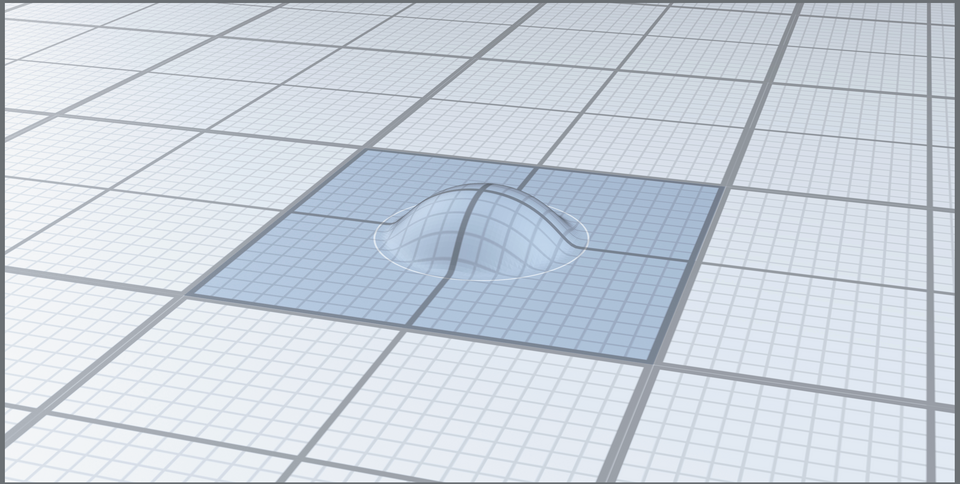
\includegraphics[scale=.8]{images/Bump.png}
\caption{by JoshDif, Wikimedia Commons, licensed under CC BY-SA 4.0}
\end{figure}
\subsection*{Exercício \theexer}
\end{frame}



\subsection*{Partição da Unidade}
\begin{frame}{Partição da Unidade}
	\begin{defin}
		Seja $X$ um subconjunto arbitrário do $\R^\dm$. Dizemos que uma cobertura aberta $(U_\lambda)_{\lambda\in \Lambda}$ de $X$ é \dt{localmente finita} se todo $x\in X$ possui  uma vizinhança $V$ que intercepta apenas um número finito de $U_\lambda$.
	\end{defin}
	
	\begin{prop}[Partição da Unidade, veja {\cite[Theorem 1.2.1]{kesavan}}]
		Seja $\Omega $ um aberto de $\R^\dm$. Dada uma cobertura aberta $(U_\lambda)_{\lambda\in \Lambda}$ de $\Omega$, existe uma família de funções   $(\theta_\lambda)_{\lambda\in \Lambda}$ definidas em $\Omega$, de classe $C^\infty$, chamada \dt{partição da unidade} subordinada à cobertura $(U_\lambda)_{\lambda\in\Lambda}$, tais que
		\begin{multicols}{2}
			\begin{enumerate}
				\item $\supp \theta_\lambda\subset U_\lambda$.
				\item $(\supp \theta _\lambda)_\lambda$ é localmente finita.
				\item $0\leq \theta_\lambda \leq 1$, para todo $\lambda \in \Lambda$.
				\item $\sum_{\lambda\in \Lambda}\theta_\lambda (x)=1$.\\
			\end{enumerate}
			
		\end{multicols}
	\end{prop}
	
\end{frame}

\begin{frame}
\begin{defin}
Sejam \(\Omega\subset \rd\) um aberto, \(K\subset V \subset \Omega\), com \(K\) compacto e \(V\) aberto. Dizemos que \(\phi:\Omega \longrightarrow \R\) é  \dt{uma função corte subordinada a \(V\) e identicamente 1 em $K$.} quando 
\[ \phi\in C_c(\Omega),\ \supp \phi \subset V,\ \phi=1 \text{ em } K \text{ e }
 0\leq \phi(x)\leq 1, \forall\, x\in \Omega.\]
\textbf{Notação do Rudin:}
\[K\prec \phi \prec V\]
%\begin{enumerate}
%\item \(K \prec \phi\)\ significa que \(K\subset \Omega\) é um compacto, \(0\leq \phi(x)\leq 1\) para todo \(x\in \Omega\), \(\phi=1\) em \(K\) e \(\phi\in C_c(\Omega)\).
%\item \(\phi \prec V\)\ significa que \(V\subset \Omega\) é um aberto, \(0\leq \phi(x)\leq 1\) e para todo \(x\in \Omega\),  \(\phi\in C_c(\Omega)\) e \(\supp \phi \subset V\).
%\item \(K\prec \phi \prec V\) quando valem os itens {\itemnum{1}} e {\itemnum{2}}. Neste caso \(\phi\)
%\end{enumerate} 
\end{defin}

\end{frame}

%%%%%%%%%%%%%%%%%%%%%%%%%%%%%%%%%%%%%%%%%%%%%%%%%%%%%%%%%%%%
\begin{frame}

\begin{corol}\label{cut-off}
Seja $K$ um compacto de $\R^\dm$. Então existem \(V\) e \(\phi\in C^\infty_c(\rd)\) tal que
\(K\prec \phi \prec V\).
\end{corol}
	\begin{proof}
		Basta considerar a partição de unidade subordinada à cobertura $(V,\R^\dm\setminus K)$, onde $V$ é um aberto limitado contendo $K$.
	\end{proof}

%\begin{exer}
%	Mostre que existe $\zeta\in C^\infty(\R^\dm)$ tal que $\zeta\equiv 1$ em $B(0,1)$ e $\supp \zeta \subset B(0,2)$.
%\end{exer}
%\subsection*{Exercício \theexer}
\end{frame}





%%%%%%%%%%%%%%%%%%%%%%%%%%%%%%%%%%%%%%%%%%%%%%%%%%%%%%%%%%
\begin{frame}{Suporte em $L^p(\Omega)$}
	\begin{defin}
Seja $u\in L^p(\Omega)$. Definimos o \dt{suporte de $u$}, denotado por {\color{blue}$\supp u$}, como o conjunto obtido pela interseção de todos os subconjuntos fechados de $\Omega$ fora dos quais {\color{blue}$u$} se anula quase sempre.
	\end{defin}

\begin{exer}
Se $u\in C^0(\Omega)\cap L^p(\Omega)$, então as duas noções de suporte coincidem. 
\subsection*{Exercício \theexer}
\end{exer}

\begin{prop}[veja {\cite[Theorem 4.12]{brezis}}]
	O espaço $C_c(\R^\dm)$ é denso em $L^p(\rd)$, para todo $1\leq p<\infty$.
\end{prop}
\end{frame}




\section{Convolução}


\subsection*{Definição de Convolução}
\begin{frame}{Convolução}
	\begin{prop}
		Dados $f,g\in L^1(\R^\dm)$, considere a função
		\[h({\color{red}x})=\int_{\R^\dm}f({\color{red}x}-y)g(y)\,dy.\]
		Então, $h$ está bem definida e pertence a $L^1(\R^\dm)$. Além disso, 
		\[\n{h}_{L^1(\R^\dm)}\leq \n{f}_{L^1(\R^\dm)}\n{g}_{L^1(\R^\dm)}.\]
	\end{prop}
	
\end{frame}
\begin{frame}
	\begin{defin}\label{def-conv}
		Dados $f,g\in L^1(\R^\dm)$ definimos a  \dt{convolução} de $f$ e $g$ por
		\[(f\ast g)({\color{red}x})=\int_{\R^\dm}f({\color{red}x}-y)g(y)\,dy.\]
	\end{defin}
	\begin{prop}
		Dados $f,g,h\in L^1(\R^\dm)$, então
		\begin{enumerate}
			\item 	$f\ast g=g*f$
			\item $(f\ast g)\ast h=f\ast(g\ast h)$
				\end{enumerate}
	\end{prop}

\end{frame}


\subsection*{Desigualdade de Young}
\begin{frame}
	\begin{prop}
		Se $f\in L^1(\R^\dm)$ e $g\in L^p(\R^\dm)$ $(1\leq p\leq +\infty)$, então $f\ast g(x)$ existe para quase todo $x$, $f\ast g\in L^p(\R^\dm)$ e  
		\[\n{f\ast g}_{L^p(\R^\dm)}\leq \n{f}_{L^1(\R^\dm)}\n{g}_{L^p(\R^\dm)}.\]
	\end{prop}
	
	\begin{teo}[Desigualdade de Young]\label{teo-young}
		Sejam $1\leq p,q,r\leq +\infty$ tais que 
		\[\frac{1}{p}+\frac{1}{q}=1+\frac{1}{r}\]
		Se $f\in L^p(\R^\dm)$, $g\in L^q(\R^\dm)$, então $f\ast g\in L^r(\R^\dm)$ e 
		\[\n{f\ast g}_{L^r(\R^\dm)}\leq \n{f}_{L^p(\R^\dm)}\n{g}_{L^q(\R^\dm)}.\]
	\end{teo}
\end{frame}

\begin{frame}
	\begin{exer}
		\begin{enumerate}
			\item 		Demonstre o Teorema \ref{teo-young}.
			
			\item Se $f$ e $g$ são funções para as quais a convolução está bem definida, então 
			\[\supp(f\ast g)\subset \supp f+\supp g.\]
		\end{enumerate}

	\end{exer}
	
	\begin{prop}
		Se $f\in C_c(\R^\dm)$ e $g\in \Lloc^1(\R^\dm)$ a integral da Definição \ref{def-conv} está bem definida para \dt{todo} $x\in \R^\dm$. Além disso, $f\ast g\in C(\R^\dm)$.
	\end{prop}

\subsection*{Exercício \theexer}
\end{frame}




\subsection*{Notação de Multi-índice}
\begin{frame}{Notação de Multi-índice}
	Considere $u:\Omega\subset \R^\dm\to \R$, $x=(x_1,\ldots,x_n)\in \R^\dm$.
	\begin{itemize}
		\item Uma n-upla $\alpha=(\alpha_1,\ldots,\alpha_\dm)$ de números inteiros não negativos é chamada de \dt{multi-índice} de ordem 
		\[|\alpha|=\alpha_1+\cdots+\alpha_\dm\]
		
		\item Definimos o operador derivação $D^\alpha$ por
		\[D^\alpha u(x)= \frac{\partial^{|\alpha|}u(x)}{\partial{x_1}^{\alpha_1} \cdots\partial{x_d}^{\alpha_d}}=\partial_1^{\alpha_1}\partial_2^{\alpha_2}\cdots\partial_\dm^{\alpha_\dm}u(x)\]
			
		\item Escrevemos  $\alpha!=\alpha_1!\alpha_2!\cdots\alpha_n!$. Diremos que $\beta\leq \alpha$, se $\beta_i\leq \alpha_i$, para $i=1,2,\ldots,n$. Com essa notação a fórmula de Leibniz é escrita como:
		\[D^\alpha(uv)=\sum_{\beta\leq \alpha}\frac{\alpha!}{\beta!(\alpha-\beta)!}(D^\beta u)(D^{\alpha-\beta} v).\]
	\end{itemize}
\end{frame}


\subsection*{Derivação da convolução}
\begin{frame}{Derivação da convolução}
		
	\begin{prop}
		Sejam  {\color{red}$f\in C_c^k(\R^\dm)$} $(k\geq 1)$ e $g\in \Lloc^1(\R^\dm)$. Então {\color{red}$f\ast g\in C^k(\R^\dm)$} e 
		\[{\color{red}D^\alpha}(f\ast g)=({\color{red}D^\alpha f})\ast g,\ \forall \alpha\in \N \text{ com } |\alpha|\leq k.\]
		Em particular, se $f\in C_c^\infty(\R^\dm)$ e $g\in \Lloc^1(\R^\dm)$, então $f\ast g\in C^\infty(\R^\dm)$.
	\end{prop}
\end{frame}

\subsection*{Funções regularizantes}
\begin{frame}{Regularização de funções \footnotemark}
		\begin{defin}
		Uma sequência de funções  $(\rho_n)_{n\in \N}$ em $\R^\dm$ são ditas \dt{funções regularizantes} quando satisfazem:
		\[\rho_n\in C_c^\infty (\R^\dm),\ \supp \rho_n \subset \overline{B_{1/n}(0)}\, \rho_n \geq 0 \ \text{ e } \int_{\R^\dm}\rho_n\, dx=1.\]
	\end{defin}
	\begin{exe}\label{seq-regul}
		Sejam $\eta:\R^\dm\longrightarrow \R$ definida como no Exemplo \ref{ex-exponencial} e \(C=\left(\int_{\rd} \eta(x)\,dx\right)^{-1}\), defina \(\rho(x)=C\eta(x)\). Para cada $\ep>0$, defina a seguinte família de funções:
		\[\textcolor{red}{\rho_\ep(x)=\frac{1}{\ep^\dm}\rho\left(\frac{x}{\ep}\right)}.\]
Tomando $\ep=1/n$, temos uma sequencia de funções regularizantes.
	\end{exe}
\footnotetext[1]{A Técnica de regularização por convolução foi originalmente introduzida por Leray e Friedrichs}
\end{frame}


\subsection*{Densidade de \texorpdfstring{$C_c^\infty(\Omega)$ em $L^p(\Omega)$}{C𞁞∞ (Ω) em L𞀾(Ω)}}
\begin{frame}{Densidade de $C_c^\infty(\Omega)$ em $L^p(\Omega)$}
	\begin{prop}
		Seja $(\rho_n)$ uma sequência de funções regularizantes. Se $f\in C(\R^\dm)$, então $\rho_n\ast f\to f$ uniformemente em cada compacto do $\R^\dm$.
		
	\end{prop}

\begin{prop}
	Seja $(\rho_n)$ uma sequência de funções regularizantes. Se $f\in L^p(\R^\dm)$, com $1\leq p<\infty$, então $\rho_n\ast f \to f$ em $L^p(\R^\dm)$, quando $n\to +\infty$.
\end{prop}

\begin{prop}\label{densLp}
	Seja $\Omega \subset \R^\dm$ um aberto. Então $C_c^\infty(\Omega)$ é denso em $L^p(\Omega)$, para todo $1\leq p<\infty$.
\end{prop}

\end{frame}

\subsection*{Lema de Du Bois Raymond}
\begin{frame}{Lema de Du Bois Raymond}
\begin{prop}[Du Bois Raymond - ver {\cite[Corollay 4.24]{brezis}} ]
	Seja $\Omega$ um aberto de $\R^\dm$. Se $u\in \Lloc^1(\Omega)$ tal que 
	\[\int_\Omega u(x)\varphi(x)\, dx=0, \ \forall \varphi\in C_c^\infty(\Omega).\]
	Então $u=0$ q.s. em $\Omega$.  
\end{prop}

\begin{exampleblock}{Lema}
Sob as hipóteses do Lema de Du Bois Raymond,
\[
\int_\Omega u(x)g(x)\,dx=0,
\]
para toda \(g\in L^\infty(\rd)\), com suporte compacto em \(\Omega\).
\end{exampleblock}

\end{frame}


\section{Distribuições}

\subsection*{Funções testes}
\begin{frame}{Funções Testes}
	\begin{defin}
		Definimos o \dt{espaço das funções testes}, denotado por $\D(\Omega)$, o conjunto $C_c^\infty(\Omega)$ dotado da seguinte noção de convergência: Dados uma sequência $(\varphi_m)$ em  $\D(\Omega)$ e $\varphi\in \D(\Omega)$, dizemos que 
		\[\varphi_m\to \varphi \text{ em } \D(\Omega),\]
		quando existe $K\subset \Omega$ compacto tal que 
		\begin{enumerate}[$i$]
			\item $\supp \varphi_m$, $\supp \varphi\subset K$, $\forall m\in \N$;
			\item $D^\alpha \varphi_m\to D^\alpha \varphi$ uniformemente em $K$, $\forall \alpha\in \N^n$.
		\end{enumerate}
	\end{defin}


	Na verdade, $\D(\Omega)$ é o espaço vetorial $C_c^\infty(\Omega)$ munido de uma topologia definida por uma família de seminormas. Esta topologia nos dá a noção de convergência  acima. Para mais detalhes, veja \cite[Appendix 2]{kesavan} ou \cite[Seção 1.3]{cavalcanti-dist}.

\end{frame}



\subsection*{Distribuições}
\begin{frame}{Distribuições sobre $\Omega$}
	\begin{defin}
		Seja $\Omega$ um aberto de $\R^\dm$.	Uma \dt{distribuição sobre $\Omega$} é um funcional linear $T:\D(\Omega)\longrightarrow \R$ que é contínua no sentido da convergência sobre $\D(\Omega)$, isto é, 
		\begin{center}
			para toda $\varphi_m\to 0$ em $\D(\Omega)$, tem-se que 
			$\inp{T}{\varphi_m}\to 0$.
		\end{center}
		
		
		O espaço das distribuições é o dual do espaço das funções testes $\D(\Omega)$ e é denotado por $\D'(\Omega)$.
	\end{defin}
\end{frame}

\begin{frame}
		\begin{exe}
		 	Se $u\in \Lloc^1(\Omega)$, então $T_u$ definida por 
				\[\inp{T_u}{\varphi}=\int_\Omega u(x)\varphi(x)\,dx, \ \varphi \in \D(\Omega)\]
				é uma distribuição sobre $\Omega$.
	
	\end{exe}
	\begin{prop}
	A aplicação $T: u\in \Lloc^1(\Omega)\longmapsto T_u \in \D'(\Omega)$ é linear, injetiva e contínua, isto é, $\Lloc^1(\Omega)\hookrightarrow \D'(\Omega)$. 	
\end{prop}

\end{frame}

\subsection*{Distribuição delta de Dirac}
\begin{frame}{Distribuição delta de Dirac}
	\begin{example}
		\begin{enumerate}
			\item 		Dado $x_0\in \Omega $, a aplicação $\delta_{x_0}$ definida por 
			\[\inp{\delta_{x_0}}{\varphi}=\varphi(x_0),\ \varphi\in \D(\Omega),\]
			é uma distribuição sobre $\Omega$ denominada \dt{delta de Dirac}\footnote{$\delta_0$ é conhecida por ``função $\delta$ de Dirac" e foi introduzida por Paul Dirac em 1930. Seus cálculos simbólicos não faziam sentido matemático até a correta formulação pela Teoria das Distribuições desenvolvida por Laurent Schwartz.}.
			
			\item A distribuição $\delta_{x_0}$ não é definida por uma função localmente integrável.
		\end{enumerate}
		
	\end{example}

\end{frame}

\begin{frame}
	\begin{exer}
		Mostre que são distribuições:
\begin{enumerate}
	\item Seja $\lambda $ um caminho retificável de classe $C^1([a,b])$ cuja imagem está contida em $\Omega$. Defina
	\[\inp{\delta_\lambda}{\varphi}=\int_\lambda \varphi\, ds,\ \forall \varphi\in \D(\Omega).\]
	
	\item Seja $v(x)=1/x,$ $x\neq 0$. Defina
	\[\inp{VP(1/x)}{\varphi}=\lim\limits_{\ep\to 0}\int_{|x|>\ep}\frac{\varphi}{x}\,dx, \ \forall \varphi\in \D(\R),\]
	denominada distribuição Valor Principal de $1/x$.
	
	\item O funcional $\varphi \in D(\Omega) \longmapsto \varphi'(0)\in \R$, conhecido como doublet ou dipole distribuition.
\end{enumerate}
	\end{exer}
\subsection*{Exercício \theexer}
\end{frame}


\subsection*{Convergência de Distribuições}

\begin{frame}{Convergência de Distribuições}
	Sendo  $\D'(\Omega)$ o  dual de um espaço vetorial topológico, podemos considerar sobre ele a topologia fraca*. Com essa topologia, temos a seguinte noção de convergência.
	
	\begin{defin}
Dizemos que $T_n\to T$ em $\D'(\Omega)$ se
\[\inp{T_n}{\varphi}\to \inp{T}{\varphi},\ \forall \varphi \in \D(\Omega).\]
	\end{defin}
	\begin{exe}
A sequência de funções regularizantes $(\rho_n)$ definidas no Exemplo \ref{seq-regul} converge para a distribuição delta de Dirac $\delta_{0}$. Isto é, uma sequência de funções localmente integráveis pode convergir para um distribuição que não é definida por uma função localmente integrável.
	\end{exe}
\end{frame}

\subsection*{Derivadas das Distribuições}
\begin{frame}{Derivadas das Distribuições}
\begin{defin}
	Sejam $T\in \D'(\Omega)$ e $\alpha\in \N^\dm$. A \dt{derivada} de ordem $\alpha$ de $T$ é a distribuição $D^\alpha T$ definida por:
	\[\inp{D^\alpha T}{\varphi}=(-1)^{|\alpha|}\inp{T}{D^\alpha \varphi},\ \forall \varphi \in \D(\Omega).\]
\end{defin}

\begin{exe}
	\begin{enumerate}[a]
		\item Se $u\in C^1(\Omega)$ então a derivada no sentido das distribuições coincide com a derivada no sentido clássico.
		
		\item Se $\Omega=(-1,1)$ então a função  
		$u(x)=\chi_{(0,1)}$ é localmente integrável, com derivada clássica $u'=0$, exceto em $x=0$, mas $Du=\delta_0$ no sentido das distribuições.
		
	\end{enumerate}
\end{exe}
\end{frame}

	
\subsection*{Derivada Fraca}
\begin{frame}
	
\begin{defin}
	Dados  $u\in \Lloc^1(\Omega)$ e $\alpha\in \N^\dm$, dizemos que $D^\alpha u\in \D'(\Omega)$ é a \dt{derivada fraca} de $u$ quando $D^\alpha u\in \Lloc^1(\Omega)$, isto é, quando existe $v\in \Lloc^1(\Omega)$ tal que 
	\[\inp{D^\alpha u}{\varphi}=\int_\Omega v\varphi\, dx, \forall \varphi\in \D(\Omega).\]
\end{defin}

\begin{prop}
Se $f$ é absolutamente contínua em $[a,b]$, então $f$ é derivável q.s. em $[a,b]$ e as derivadas clássicas e distribucional coincidem.
\end{prop}

\begin{prop}
	Se $T_n\to T$ em $\D'(\Omega)$, então $D^\alpha T_n\to D^\alpha T$ em $\D'(\Omega)$, para qualquer multi-índice $\alpha$. Em outras palavras, o operador $D^\alpha: \D'(\Omega) \longrightarrow \D'(\Omega)$ é linear e contínuo.
\end{prop}
\end{frame}

\subsection*{Multiplicação de distribuições por funções $C^\infty$}
\begin{frame}{Multiplicação de distribuições por funções $C^\infty$}
\begin{defin}
	Sejam $T\in \D'(\Omega)$ e $\psi\in C^\infty(\Omega) $. O \dt{produto $\psi T$} por:
	\[\inp{\psi T}{\varphi}=\inp{T}{\psi \varphi},\ \forall \varphi\in \D(\Omega) \]
	define uma distribuição sobre $\Omega$.
\end{defin}

\begin{exer}
	Prove a fórmula de Leibniz para distribuições: 	Seja $\Omega\subset \R^\dm$ um aberto. Se $\psi\in C^\infty(\Omega)$ e $T\in \D'(\Omega)$, então
	\[D^\alpha(\psi T)=\sum_{\beta\leq \alpha}\frac{\alpha!}{\beta!(\alpha-\beta)!}D^\beta\psi D^{\alpha-\beta}T,\ \forall \alpha\in \N^\dm.\]
\end{exer}
\subsection*{Exercício \theexer}
\end{frame}


\section{Espaços de Sobolev}

\subsection*{Espaços de Sobolev}
\begin{frame}{Espaços de Sobolev}
\begin{defin}
 Sejam $\Omega \subset \R^\dm$, {\color{blue}$k\geq 0$} um inteiro e {\color{red}$1\leq p\leq +\infty$}. O \dt{Espaço de Sobolev} $W^{{\color{blue}k},{\color{red}p}}(\Omega)$  é o espaço vetorial normado definido por 
 \[W^{{\color{blue}k},{\color{red}p}}(\Omega):=\{u\in L^{\color{red}p}(\Omega);\ D^{\color{blue}\alpha} u\in L^{\color{red}p}(\Omega),\ \forall\, {\color{blue}|\alpha|\leq k}\},\]
 com a norma dada por 
 \[
 \n{u}_{{\color{blue}k},{\color{red}p},\Omega}=
\begin{cases}
\displaystyle\left(\sum_{{\color{blue}|\alpha|\leq k}} \n{D^{\color{blue}\alpha} u}^{\color{red}p}_{L^{\color{red}p}(\Omega)}\right)^{1/{\color{red}p}}, & \text{ se } {\color{red}p\in [1,+\infty)}\\[2em]
\displaystyle\sum_{{\color{blue}|\alpha|\leq k}} \n{D^{\color{blue}\alpha} u}_{L^{\color{red}\infty}(\Omega)}, & \text{ se } {\color{red}p=\infty}
\end{cases}
\]

\end{defin}



\end{frame}

\begin{frame}
	\begin{block}{Notações}
		\begin{enumerate}
			
			\item Note que $W^{0,p}(\Omega)=L^p(\Omega)$ e  $\n{u}_{0,p,\Omega}=\n{u}_{L^p(\Omega)}$ que denotaremos simplesmente por $\n{u}_{p,\Omega}$.
			
			\item Quando não houver perigo de confusão omitiremos $\Omega$ na notação da norma.
			
			
		\item   Se $p=2$, escrevemos $H^k(\Omega)=W^{k,2}(\Omega)$. 
		\end{enumerate}
	\end{block}

	\begin{exer}
	Mostre que $W^{k,p}(\Omega)$ é um espaço vetorial normado e que  $\n{u}_{k,p,\Omega}$ é equivalente à norma
	\[\n{u}=\sum_{|\alpha|\leq k}\n{D^\alpha u}_{L^p(\Omega)}.\]
\end{exer}
\end{frame}

\begin{frame}
	\begin{exe}
\begin{enumerate}[a]
	\item Sejam $\Omega=(-1,1)$ e	$u(x)=x\chi_{(0,1)}$. Note que $u\in L^1(-1,1)$, $u'\in L^1(-1,1)$ no sentido clássico, mas $Du=\delta_0\not\in L^1(-1,1)$ (não possui derivada fraca), portanto $u\not\in W^{1,1}(-1,1)$.
	
	\item Sejam $\Omega=B(0,1)$, $\alpha>0$ e $u(x)=\|x\|^{-\alpha}$, $x\in \Omega$, $x\neq 0$. Mostre que $u\in W^{1,p}(\Omega)$ se, e somente se, $0<\alpha<\frac{N-p}{p}$.
\end{enumerate}

	\end{exe}

\subsection*{Exercício \theexer}
\end{frame}


\begin{frame}
	\begin{prop}
	Para todo $1\leq p\leq +\infty$, $W^{k,p}(\Omega)$ é um espaço de Banach. Se $1<p<+\infty$ ele é reflexivo e se $1\leq p<+\infty$ é separável.
\end{prop}

\begin{lema}
	Sejam $\Omega$ um aberto de $\R^\dm$ e $1\leq p\leq +\infty$. A aplicação 
	\[u\in W^{1,p}(\Omega)\longmapsto (u,\partial_1 u,\ldots,\partial_\dm u)\in L^p(\Omega)^{\dm+1}\]
	é uma \textcolor{red}{ isometria}, onde estamos munindo o espaço $L^p(\Omega)^{\dm+1}$ com a norma
	\[\n{v}=\left(\sum_{i=1}^{\dm+1}\n{v_i}_{p,\Omega}^p\right)^{1/p}\]
\end{lema}
\end{frame}

%%%%%%%%%%%%%%%%%%%%%%%%%%%%%%%%%%%%%%%%%%%%%%%%%%%%%%%%%%%%%%%%%%%%%%
\subsection*{O espaço \texorpdfstring{\(W_0^{1,p}(\Omega)\)}{W₀¹ 𞀾(Ω)}}

\begin{frame}{Espaços $W_0^{k,p}(\Omega)$}
Como vimos na Proposição \ref{densLp}, $\D(\Omega)$ é denso em $L^p(\Omega)$, mas isto não é verdade para $W^{k,p}(\Omega)$. Por essa razão, define-se o espaço 
\[W_0^{k,p}(\Omega):=\overline{\D(\Omega)}^{\|\cdot\|_{k,p}}.\]

Quando $p=2$, escrevemos $H_0^k(\Omega)$ no lugar de $W^{k,2}_0(\Omega)$. 

\begin{exer}
Sejam \(1<{\color{blue} p }<+\infty\),  \(\Omega\) um aberto de \(\rd\) e \(u\in W_0^{1,{\color{blue} p }}(\Omega)\). Mostre que \(\tilde{u}\in W^{1,{\color{blue} p }}(\rd)\), onde  \(\tilde{u}\) é a extensão de \(u\) a zero fora de \(\Omega\). Além disso, 
\[
\partial_i \tilde{u}=\widetilde{\partial_i u},\ i=1,\ldots, \dm.
\]
\end{exer}
\subsection*{Exercício \theexer}
\end{frame}

\begin{frame}

\begin{prop}
 Sejam $1\leq p<+\infty$ e $k\geq 0$ um inteiro. Então $W_0^{k,p}(\R^\dm)=W^{k,p}(\R^\dm)$.
\end{prop}

\begin{lemaaux}
	Sejam $\rho\in C_c^\infty(\R^\dm)$ e $v\in W^{1,p}(\R^\dm)$, $1\leq p< +\infty$. Então 
	\[\rho\ast v\in C^\infty(\R^\dm) \cap W^{1,p}(\R^\dm), \text{ e } \partial_i(\rho\ast v)=\rho\ast \partial_i v,\  \forall i=1,\ldots,N.\]
\end{lemaaux}
\end{frame}

\subsection*{Aproximação por Funções Suaves}

\begin{frame}{Aproximação por Funções Suaves}
	
Dados $\Omega\subset \R^\dm$ uma aberto e $\ep>0$, defina $\Omega_\ep=\{x\in \Omega;\ \operatorname{dist}(x,\partial \Omega)>\ep\}$. Dado $u\in L^p(\Omega)$ denotemos por $\tilde{u}$ a extensão a zero de $u$. Se $\rho\in C^\infty_c(\R^n)$, defina
\[\rho\ast u(x)=\rho\ast \tilde{u}(x),\ \forall x\in \Omega.\]

	
	\begin{prop}
		Sejam $\Omega \subset \R^\dm$ um aberto e $u\in W^{k,p}(\Omega)$, com $1\leq p<+\infty$, e seja $(\rho_n)$ uma sequência regularizante. Então,
		\begin{enumerate}
			\item 	$u_n=\rho_n\ast u \in C^\infty(\Omega)$ e $D^\alpha u_n=D^\alpha \rho_n\ast u$ em $\Omega$, para todo $\alpha\in \N$, $|\alpha|\leq k$.
			
			\item $u_n\to u$ em $L^p(\Omega)$.
			
			\item Dado $\ep>0$, $D^\alpha u_n =\rho_n\ast D^\alpha u$ em $\Omega_\ep$, para $n$ suficientemente grande,  $\forall \alpha\in \N$, $|\alpha|\leq k$.
		\end{enumerate}
	
	\end{prop}
	
\end{frame}

\begin{frame}{Aproximação Local por funções suaves}
\begin{teo}[Friedrichs]
	Sejam $\Omega \subset \R^\dm$ um aberto e $u\in W^{k,p}(\Omega)$ com $1\leq p<+\infty$. Então, existe uma sequência $(v_n)$ em $\D(\R^\dm)$ tal que:
	\begin{equation*}
		\begin{split}
			&	v_n\to u \text{ em } L^p(\Omega);\\		
			&	D^\alpha v_n \to  D^\alpha u, \text{ em } L^p(\Omega') \text{ para todo } \Omega'\subset\subset \Omega,\  \forall \alpha\in \N,\ |\alpha|\leq k. 
		\end{split}
	\end{equation*}
\end{teo}


\end{frame}

\subsection*{Regra da Cadeia}
\begin{frame}{Regra da Cadeia}
	\begin{prop}[Regra da Cadeia]
		Seja $G\in C^1(\R)$ tal que $G'\in L^{\infty}(\R)$. Se $u\in W^{1,p}(\Omega)$, então $G\circ u\in W^{1,p}(\Omega)$ e 
		\[\partial_i (G\circ u)=(G'\circ u)\partial_i u,\ 1\leq i\leq N.\]
	\end{prop}
	


\end{frame}


%\begin{frame}
%	
%	\begin{teo}[Rademarcher]
%		Seja $\Omega$ um aberto do $\R^\dm$.	Se $G:\Omega \to \R$ é Lipschitz contínua, então $G$ é diferenciável quase sempre em $\Omega$.
%	\end{teo}
%	
%		\begin{teo}[Regra da Cadeia - {\cite[Th. 2.1.11]{Ziemer}} ]
%		Sejam $G:\R\longrightarrow  \R$ uma função Lipschitziana e $1\leq p$. Se $u\in W^{1,p}(\Omega)$ e  $G\circ u\in L^p(\Omega)$, então $G\circ u\in W^{1,p}(\Omega)$ e
%		\[\partial_i (G\circ u)=(G'\circ u)\partial_i u,\ 1\leq i\leq N.\]
%	\end{teo}
%\end{frame}



\begin{frame}{Aproximação global por funções suaves}
\begin{teo}[Meyers-Serrin{\footnotemark[1]}]
	Sejam $\Omega\subset\R^\dm$ um aberto e \textcolor{red}{limitado} e $u\in W^{k,p}(\Omega)$, com $1\leq p<+\infty$. Então 
	\[C^\infty(\Omega)\cap W^{k,p}(\Omega) \text{ é denso em }  W^{k,p}(\Omega),\]
	isto é,  existe uma sequência de funções $(u_n)$ em $C^\infty(\Omega)\cap W^{k,p}(\Omega)$ tal que 
	\[u_n\to u \text{ em } W^{k,p}(\Omega).\]
\end{teo}

\footnotetext{N. Meyers and J. Serrin, H=W, \textit{Proc. Nat. Acad. Sci. USA} \textbf{51} (1964), 1055 -- 1056. \href{https://doi.org/10.1073/pnas.51.6.1055}{doi:10.1073/pnas.51.6.1055}
}
\end{frame}

\begin{frame}
	\begin{obs}
			Nenhum desses casos se estendem para $p=\infty$. Vejamos um exemplo simples. Considere $\Omega=(-1,1)$ e $u(x)=x\chi_{(0,1)}$. Então $u\in W^{1,+\infty}(\Omega)$ mas não pode ser aproximado por funções suaves.
	\end{obs}

\begin{prop}
	Sejam $1\leq p<+\infty$ e $u\in W^{1,p}(\Omega)$. Se $u$ tem suporte compacto, então $u\in W^{1,p}_0(\Omega)$.
\end{prop}

%\begin{teo}[Stampachia{\footnotemark[1]} - Regra da Cadeia em $W_0^{1,p}(\Omega)$]
%	Seja $G:\R\longrightarrow  \R$ uma função Lipschitziana tal que $G(0)=0$. Se $\Omega$ é um aberto \textcolor{red}{limitado} de $\R^\dm$ e $u\in W^{1,p}_0(\Omega)$, então $G\circ u\in W^{1,p}_0(\Omega)$.
%\end{teo}
%
%\footnotetext{Stampacchia, Guido. ``Equations elliptiques du second ordre à coefficients discontinus." Séminaire Jean Leray 3 (1966): 1-77. \href{http://www.numdam.org/item/SJL_1963-1964___3_1_0/}{www.numdam.org/item/SJL$\_$1963-1964}}

\end{frame}



\subsection*{Operador Prolongamento}

\begin{frame}{Operador Prolongamento}
	\begin{defin}
		Seja $\Omega$ um aberto do $\R^\dm$. Um \dt{operador prolongamento} $P$ para $W^{1,p}(\Omega)$ é um operador linear limitado
		\[P:W^{1,p}(\Omega)\to W^{1,p}(\R^\dm),\]
		tal que $Pu\vert_\Omega =u$ para toda $u\in W^{1,p}(\Omega)$.
	\end{defin}

	Seja $x\in \R^\dm$, vamos escrever $x=(x',x_\dm)$, onde $x'=(x_1,\ldots,x_{\dm-1})$ e 
	\begin{align*}
	& \R^\dm_+=\{x\in \R^\dm;\ x_\dm>0\},\\
	& Q_r=\{(x',x^\dm);\ \|x'\|<r \text{ e } |x_\dm|<r\},\\
	& Q_r^+=Q_r\cap \R^\dm_+,\\
	& Q_r^0=\{x\in Q_r; x_\dm=0\},\\
	& Q_r^{-}=\{x\in Q_r; x_\dm<0\}.
\end{align*}

\end{frame}


\subsection*{Carta local}
\begin{frame}{Carta local}
\begin{defin}
	Seja $\Omega\subset \R^\dm$ um aberto. Dizemos que {\color{red}\(\partial \Omega\) é de classe $C^k$} ($k\geq 1$ inteiro) se para cada $x\in {\color{red} \partial \Omega }$, existem {\color{blue} \(r>0\)},  uma vizinhança {\color{blue}$U$} de $x$ em $\R^\dm$ e uma aplicação {\color{blue}$\varphi:Q_r\longrightarrow U$}  tal que 
	\begin{enumerate}
		\item{\color{blue} $\varphi$} é uma bijeção.
		\item ${\color{blue}\varphi}\in C^k(\overline{Q_r})$, ${\color{blue}\varphi^{-1}}\in C^k(\overline{U})$.
		\item ${\color{blue}\varphi}(Q_r^+)=U\cap \Omega$, ${\color{blue}\varphi}(Q_r^0)=U\cap \partial \Omega$.
	\end{enumerate}
Dizemos que o par {\color{blue} \((U, \varphi)\)} é chamada uma {\color{blue}carta local} de {\color{red} \(\partial \Omega\)}.
\end{defin}

\begin{obs}
Cabe ressaltar que, por {\color{blue} \(\varphi\)} ser um difeomorfismo, podemos trocar {\color{blue} \(Q_r\)} por qualquer aberto de \(\rd\).
\end{obs}


\end{frame}


\begin{frame}
	\begin{teo}
		Seja $\Omega\subset \R^\dm$ um {\color{red} aberto com fronteira $\partial \Omega$ {de classe $C^1$} e limitada } ou \(\Omega={\color{red} \rd_{+} }\). Então, dado \( p\in [1,+\infty]\) existe um operador prolongamento $P:W^{1,p}(\Omega)\longrightarrow W^{1,p}(\R^\dm)$.
		\medskip
		
		Se, além disso, {\color{red} \(\Omega\) for limitado}, então dado um {\color{red} aberto limitado  } \(\Omega' \supset\supset \Omega \), tem-se que
		\[ \supp(Pu)\subset \Omega',\ \forall\, u\in W^{1,p}(\Omega). \]
	\end{teo}

\begin{obs}
Um exemplo de aberto {\color{blue} ilimitado},  com fronteira de classe \(C^1\) limitada, é \(\rd\setminus B(0,1)\). 
\end{obs}
\end{frame}

\begin{frame}
	\begin{corol}
Seja \(\Omega\subset \rd \) um aberto {\color{red} com fronteira de classe \(C^1\) limitada}. Então o subespaço de \(\cc({\rd})\) formado pelas restrições em \(\Omega\) é um subespaço denso de \( W^{1,p}(\Omega)\), com \(1\leq p<\infty\). Precisamente, se \(u\in W^{1,p}(\Omega)\), então existe \((u_n)_{n\in \N}\subset C^\infty_c(\R^\dm)\) tal que 
\[u_n\big\vert_\Omega\longrightarrow u \text{ em } W^{1,p}(\Omega).\]
Em particular, \(C^\infty(\overline{\Omega})\) é denso em \(W^{1,p}(\Omega)\), sempre que \(\Omega\subset \rd \) é um aberto  {\color{red} com fronteira limitada de classe \(C^1\)}.
	\end{corol}
	
\end{frame}

\begin{frame}{Prova do Teorema do Prolongamento: Método de reflexão}


Dado $u:Q_1^+\longrightarrow \R$, denote $u^\ast:Q_1\longrightarrow$ \dt{a extensão  por reflexão} de $u$, isto é,
\[u^\ast(x',x^\dm)=\begin{cases}
	u(x',x^\dm), & x^\dm>0,\\ u(x',-x^\dm), & x^\dm<0.
\end{cases}\]
	
	\begin{lema}
		Seja $u\in W^{1,p}(Q_1^+)$ (ou $ W^{1,p}(\R^\dm_+)$), com $1\leq p\leq +\infty$. Então $u^\ast\in W^{1,p}(Q_1)$ (ou $ W^{1,p}(\R^\dm)$) e 
		\[\n{u^\ast}_{p,Q_1}\leq 2\n{u}_{p,Q_1^+} \text{ e } \n{u^\ast}_{1,p,Q_1}\leq 2\n{u}_{1,p,Q_1^+}.\]
		Em particular, $P:u\in W^{1,p}(\R_+^\dm) \longmapsto u^\ast \in W^{1,p}(\R^\dm)$, define um operador prolongamento.
	\end{lema}
	
	
\end{frame}




\subsection*{Traço}

%%%%%%%%%%%%%%%%%%%%%%%%%%%%%%%%%%%
\begin{frame}{Teorema do Traço}


\begin{teo}[Caso \(\Omega=\rd_+\)] 
Existe um operador linear contínuo \(\gamma_0: W^{1,p}(\rd_+)\longrightarrow L^p(\R^{d-1})\), denominado {\color{blue} operador traço}, tal que 
se \(u\in C^0(\overline{\rd_+})\), então \(\gamma_0(u)=u\big\vert_{\R^{d-1}}\).
\end{teo}

\begin{teo} 
Seja $\Omega\subset \R^\dm$ um {\color{blue} aberto limitado} {\color{red} com fronteira {de classe $C^1$}}. Então existe um operador linear contínuo \(\gamma_0: W^{1,p}(\Omega)\longrightarrow L^p(\partial \Omega)\), denominado {\color{blue} operador traço}, satisfazendo:
Se \(u\in C^0(\overline{\Omega})\), então \(\gamma_0(u)=u\big\vert_{\partial\Omega}\).
\end{teo}

\end{frame}

%%%%%%%%%%%%%%%%%%%%%%%%%%%%%%%%%%%
\begin{frame}
\begin{teo}[Fórmula de Integração por Partes]
Seja \(\Omega\subset \rd\) um {\color{blue} aberto limitado } {\color{red} com fronteira de classe \(C^1\)}. Então, 
\[
\int_\Omega u\,\partial_iv\, dx
=-\int_\Omega \partial_i u\, v\, dx
+\int_{\partial \Omega} \gamma_0(u)\gamma_0(v)\nu^i\, dS(x), 
\] 
para toda \(u\in W^{1,p}(\Omega), v\in W^{1,p'}(\Omega)\), onde \(\nu^i\) é a \(i-\)ésima coordenada o vetor normal \(\nu\) apontando para fora de \(\Omega\). 
\end{teo}


\begin{teo} 
Seja $\Omega\subset \R^\dm$ um {\color{red} aberto limitado {de classe $C^1$}} ou \(\Omega=\rd_+\). Então
\[\ker( \gamma_0 )=W_0^{1,p}(\Omega).\]
\end{teo}

\end{frame}

%%%%%%%%%%%%%%%%%%%%%%%%%%%%%%%%%%%

\subsection*{Traço Geral Espaços de Hilbert}
\begin{frame}{Teorema do Traço Geral caso \(p=2\)}
\begin{teo}
Seja \(\Omega\subset \rd\) um {\color{blue} aberto limitado } {\color{red} com fronteira de classe \(C^1\)}. Então existe um operador  linear e contínuo \(\gamma: H^k(\Omega)\longrightarrow (L^2(\Omega))^k\), denominado {\color{blue}operador traço}, onde \(\gamma=(\gamma_0,\gamma_1,\ldots,\gamma_{k-1})\), satisfazendo
\begin{enumerate}
\item Se \(u\in C^{k-1}(\overline{\Omega})\), então \(\gamma_0(u)=u\big\vert_{\partial \Omega}\) e  \(\gamma_i(u)=\partial_iu\big\vert_{\partial \Omega}\), \(i=1,\ldots,k-1\).

\item  \(\ker(\gamma)=H_0^k(\Omega).\)
\end{enumerate}
\end{teo}



\end{frame}

%%%%%%%%%%%%%%%%%%%%%%%%%%%%%%%%%%%
\section{Imersões de Sobolev}

\begin{frame}{Imersões de Sobolev}
	
\begin{defin}
	Sejam \(E\) e \(F\) espaços vetoriais normados. Dizemos que \(E\) está  \dt{imerso continuamente} em \(F\), quando existe uma aplicação linear {\color{red}injetora} \(T:E\longrightarrow F\), que também é contínua, isto é, existe \(C>0\) tal que
	\[\n{T(u)}_F\leq C \n{u}_E.\]
\end{defin}	

No caso particular das imersões de Sobolev, {\color{blue}\(T\) será sempre a inclusão} entre um mesmo espaço vetorial \(X\) com normas diferentes, isto é \(E=(X,\|\cdot \|_E)\) e \(F=(X,\|\cdot\|_F)\), a qual é sempre injetora, bastando verificar apenas que 
\[\|u\|_F\leq C\|u\|_E.\]	
Neste caso, esta imersão será denotada  por {\color{blue} \(E\hookrightarrow F\)}.

\end{frame}

\begin{frame}
\begin{exampleblock}{Pergunta}
%	Se uma função \(u\in {\color{blue}W^{1,p}(\Omega)}\), então \(u\) pertence automaticamente a algum outro espaço \({\color{red}X}\)? Em outras palavras, \( {\color{blue}W^{1,p}(\Omega)}\subset {\color{red}X}\)? 
Existe algum espaço  \({\color{red}X}\) para o qual temos automaticamente que  \({\color{blue}W^{1,p}(\Omega)}\hookrightarrow {\color{red} X }\)?
\end{exampleblock}	
A resposta é sim! Mas o espaço \({\color{red}X}\) depende de quando:
\begin{equation*}
	\begin{split}
1\leq {\color{blue}p}<\dm, \\ {\color{blue}p}=\dm, \\ \dm<{\color{blue}p}\leq \infty.
	\end{split}
\end{equation*}	
\end{frame}

\subsection*{Desigualdade de Gagliardo-Nirenberg-Sobolev}
\begin{frame}{Caso \(\Omega=\rd\) e \(1\leq p<\dm\)}
	Começemos pelo caso \(1\leq p<\dm\) e \(\Omega=\rd\). Neste caso, veremos que 
	\[{\color{blue}W^{1,p}(\rd)}\hookrightarrow {\color{red} L^q(\rd)},\]
para algum \({\color{red} q}\).

\begin{block}{Argumento de Reescala}
	A fim de encontrarmos um candidato à {\color{red} \(q\) }, tome \(u\in \cc(\rd)\) e defina
	\[u_\lambda(x)=u(\lambda x).\]
	Suponha que 
	\[\n{u_\lambda}_{{\color{red} q },\rd}\leq C \n{\nabla u}_{p,\rd}.\]
\end{block}
\end{frame}

\begin{frame}{Expoente conjugado de Sobolev}
Definimos o {\color{red}expoente conjugado de Sobolev de} \({\color{blue} p }\in [1,\dm)\) por
	\[{\color{red} p^\ast }:=\frac{\dm {\color{blue} p }}{\dm - {\color{blue} p }}.\]
Note que 
\[\frac{1}{{\color{red} p^\ast }}=\frac{1}{{\color{blue} p }}-\frac{1}{\dm}\ \  \text{ e }\ \  {\color{red}  p^\ast }>{\color{blue} p }.\]


\end{frame}

\begin{frame}{Desigualdade de Gabliardo-Nirenberg-Sobolev}
\begin{teo}[{Gabliardo-Nirenberg-Sobolev}]\label{GNS}
Se \(1\leq{\color{blue}  p }< \dm\), então \(W^{1,{\color{blue} p }}(\rd)\subset L^{{\color{red} p^\ast }}(\rd)\) e existe uma constante \(C=C_{{\color{blue} p },\dm}>0\) tal que 
\begin{equation*}
\n{u}_{{\color{red} p^\ast },\rd}\leq C\n{\nabla u}_{{\color{blue} p },\rd}
\end{equation*}
\end{teo}
\begin{exampleblock}{Passos da Prova}
\begin{enumerate}
\item Provar para \(u\in C^1_c(\rd)\).
\begin{itemize}
\item Caso \(p=1\): TFC + Desigualdade de Hölder + integrações sucessivas.
\item Caso \(p>1\): Aplicar caso anterior para \(v=|u|^\gamma\), com \(\gamma=\frac{p(\dm -1)}{\dm-p}\).
\end{itemize}
\item Usar a densidade de \(\cc(\rd)\) em \(W^{1,p}(\rd)\)
\end{enumerate}
\end{exampleblock}

\end{frame}


\begin{frame}

\begin{corol}
Se \(1\leq {\color{blue} p }<\dm \), então
\[W^{1,{\color{blue} p }}(\rd)\hookrightarrow L^q(\rd), \ \forall q\in [{\color{blue} p },{\color{red} p^\ast }].\]
\end{corol}


\begin{exampleblock}{Desigualdade de Interpolação para normas \(L^p\) {\cite[Appendix B.2(h)]{evans}}}
Sejam \(\Omega\subset \rd\) um aberto e \(1\leq p\leq q\leq \infty\). Se \(u\in L^p(\Omega)\cap L^q(\Omega)\), então \(u\in L^r(\Omega)\) para todo \(r\in [p,q]\) e 
\[
\n{u}_{r,\Omega}\leq \n{u}^\theta_{p,\Omega}\n{u}_{q,\Omega}^{1-\theta},
\]
onde
\[
\frac{1}{r}=\frac{\theta}{p}+\frac{(1-\theta)}{q}
\]
\end{exampleblock}

\end{frame}

\begin{frame}{Caso \(\Omega=\R^\dm\) e \(p=\dm\)}
\begin{corol}
Se \({\color{blue} p }=\dm\), então
\[
W^{1,{\color{blue}p}}(\rd) \hookrightarrow L^{\color{red} q }(\rd),\ \forall {\color{red} q }\in [\dm,+\infty).
\]
\end{corol}

\begin{exampleblock}{}
Usaremos a seguinte desigualdade obtida na prova do Teorema \eqref{GNS}:

 \(\forall{\color{blue}  \gamma }>1 \), temos que
\[
{\color{red} \n{u}_{{\frac{{\color{blue} \gamma}\dm}{\dm-1}}}}
\leq {\color{blue} \gamma }
{\color{red} \n{u}^{{\color{blue} \frac{1}{\gamma'}}}_{p'(\gamma-1)}}\n{\nabla u}_p^{{\color{blue} \frac{1}{\gamma}}},\ \forall u\in \cc(\rd).
\]
\end{exampleblock}

\end{frame}

%%%%%%%%%%%%%%%%%%%%%%%%%%%%%%%%%%%%%%%%%%%%%%%%%%%%%%%%%%%%%%%%%%%%%%%%
\subsection*{Desigualdade Morrey}
\begin{frame}{Caso \(\Omega=\R^\dm\) e \(p>\dm\)}
\begin{teo}[Desigualdade de Morrey]
Se \({\color{blue} p }>\dm\), então existe \(C=C_{{\color{blue}p},\dm}>0\) tal que  para toda \( u\in W^{1,{\color{blue} p }}(\rd) \) vale
\[
|u(x)-u(y)|\leq C|x-y|^{{\color{red} \gamma }} \n{\nabla u}_{1,{\color{blue} p },\rd} \text{ q.t.p } x,y\in \rd.
\]
onde \({\color{red} \gamma }:=1-\dm/{\color{blue} p }\).
Consequentemente, 
\[
\n{u}_{C^{0,{\color{red} \gamma }}(\rd)}\leq C \n{u}_{1,{\color{blue}p},\rd}\, \forall u\in W^{1,{\color{blue} p }}(\rd),
\]
o que significa que
\[
W^{1,{\color{blue}p}}(\rd) \hookrightarrow C^{0,{\color{red} \gamma }}(\rd).
\]
\end{teo}

%\begin{exampleblock}{Integral sobre hipersuperfícies em \(\rd\)}
%\[
%\int_M f(x)\, dx = \int_U f(x(u)) |\det[\frac{\partial x}{\partial u_1}]|
%\]
%\end{exampleblock}
\end{frame}

%%%%%%%%%%%%%%%%%%%%%%%%%%%%%%%%%%%%%%%%%%%%%%%%%%%%%%%%%%%%%%%%%%%%%%%%%%

%%%%%%%%%%%%%%%%%%%%%%%%%%%%%%%%%%%%%%%%%%%%%%%%%%%%%%%%%%%%%%%%%%%%%%%%
\subsection*{Imersões de Sobolev Geral}
\begin{frame}{Caso \(\Omega=\R^\dm\): Imersão Geral}
\begin{teo}[Imersão de Sobolev Geral] Para todo \(k\geq 1\) e \({\color{blue} p }\in [1,+\infty]\)
\begin{align*}
& W^{k,{\color{blue} p }}(\rd)\hookrightarrow L^{\color{red} q }(\rd), \text{ com } \frac{1}{{\color{red} q }}=\frac{1}{{\color{blue} p }}-\frac{k}{\dm},  &
 \text{ se } k{\color{blue} p }<\dm,\\
%--------------------------------------
& W^{k,{\color{blue} p }}(\rd)\hookrightarrow L^{\color{red} q }(\rd),\ \forall {\color{red} q }\in [{\color{blue} p },+\infty),& \text{ se }  k{\color{blue} p }=\dm,\\
& W^{k,{\color{blue} p }}(\rd)\hookrightarrow C^{{\color{red} m },{\color{red} \gamma }}(\rd),
%\text{ com }
%{\color{red}m}:=\bigg\lfloor k-\frac{\dm}{{\color{blue} p }}\bigg\rfloor 
%\text{ e } {\color{red} \gamma }=  \operatorname{frac}\left(k-\frac{\dm}{{\color{blue} p}}\right) 
& \text{ se }  k{\color{blue} p }>\dm,
\end{align*}
onde 
\[
\begin{cases}
{\color{red}m}:= k-\frac{\dm}{{\color{blue} p}} 
\text{ e } 0< {\color{red} \gamma }<1,
& \text{ se } k-\frac{\dm}{{\color{blue} p }} \text{é inteiro},\\
{\color{red}m}:=\bigg\lfloor k-\frac{\dm}{{\color{blue} p }}\bigg\rfloor 
\text{ e } {\color{red} \gamma }=  \operatorname{frac}\left(k-\frac{\dm}{{\color{blue} p}}\right), 
& \text{ se } k-\frac{\dm}{{\color{blue} p }} \text{ não é inteiro},
\end{cases}
\]
onde \(\lfloor\cdot \rfloor\) é a parte inteira de um número e \(\operatorname{frac(\cdot)}\) é a sua parte fracionária, isto é, \(\operatorname{frac}(x)=x-\lfloor x\rfloor\). A constante de imersão depende apenas de \(k, {\color{blue} p }\) e \(\dm\).
\end{teo}


\end{frame}

%%%%%%%%%%%%%%%%%%%%%%%%%%%%%%%%%%%%%%%%%%%%%%%%%%%%%%%%%%%%%%%%%%%%%%%%%%

\begin{frame}

\begin{exer}
Provar este resultado. Basta aplicar os resultados anteriores indutivamente. Ver \cite{evans}.
\end{exer}
\subsection*{Exercício \theexer}

\begin{exe}
\begin{enumerate}
\item \(W^{1,\infty}(\rd)\hookrightarrow C^{0,1}(\rd)\). Por isso as funções de  \(W^{1,\infty}(\rd)\) são chamadas de Lipschtzianas.
\item \(W^{1,p}(\R)\hookrightarrow C^{0,\frac{1}{2}}(\R)\), para todo \(p>1\). 

\item  \(W^{1,1}(\R)\hookrightarrow L^q(\R) \), para todo \(q\geq 1\). 

\item \(H^k(\rd)\hookrightarrow C^0(\rd)\) para \(2k>\dm\). 

\item  Se \(u\in W^{k,p}(\rd)\) para todo \(k>0\), então \(u\in C^\infty(\rd)\).
\end{enumerate}
\end{exe}
\end{frame}

%%%%%%%%%%%%%%%%%%%%%%%%%%%%%%%%%%%%%%%%%%%%%%%%%%%%%%%%%%%%%%%%%%%%%%%%%%

\subsection*{Caso \texorpdfstring{\(\Omega\subset\rd\)}{Ω⊂ℝᵈ}}
\begin{frame}{O caso \(\Omega\subset\rd\)}
\begin{teo}
Seja \(\Omega\) um aberto de \(\rd\), {\color{red} com fronteira limitada \(C^1\)} ou \(\Omega={\color{red} \rd_{+} }\). Para todo \(k\geq 1\) e \({\color{blue} p }\in [1,+\infty]\)
\begin{align*}
& W^{k,{\color{blue} p }}(\Omega)\hookrightarrow L^{\color{red} q }(\Omega), \text{ com } \frac{1}{{\color{red} q }}=\frac{1}{{\color{blue} p }}-\frac{k}{\dm},  &
 \text{ se } k{\color{blue} p }<\dm,\\
%--------------------------------------
& W^{k,{\color{blue} p }}(\Omega)\hookrightarrow L^{\color{red} q }(\Omega),\ \forall {\color{red} q }\in [{\color{blue} p },+\infty),& \text{ se }  k{\color{blue} p }=\dm,\\
& W^{k,{\color{blue} p }}(\Omega)\hookrightarrow C^{{\color{red} m },{\color{red} \gamma }}(\Omega),
%\text{ com } {\color{red}m}:=\bigg\lfloor k-\frac{\dm}{{\color{blue} p }}\bigg\rfloor 
% \text{ e } {\color{red} \gamma }=  \operatorname{frac}\left(k-\frac{\dm}{{\color{blue} p}}\right)   ,   
& \text{ se }  k{\color{blue} p }>\dm,
\end{align*}
onde 
\[
\begin{cases}
{\color{red}m}:= k-\frac{\dm}{{\color{blue} p}} 
\text{ e } 0< {\color{red} \gamma }<1,
& \text{ se } k-\frac{\dm}{{\color{blue} p }} \text{é inteiro},\\
{\color{red}m}:=\bigg\lfloor k-\frac{\dm}{{\color{blue} p }}\bigg\rfloor 
\text{ e } {\color{red} \gamma }=  \operatorname{frac}\left(k-\frac{\dm}{{\color{blue} p}}\right), 
& \text{ se } k-\frac{\dm}{{\color{blue} p }} \text{ não é inteiro},
\end{cases}
\]
A constante de imersão depende apenas de \(k, {\color{blue} p }, \dm\) e \(\Omega\).
\end{teo}
\end{frame}


%%%%%%%%%%%%%%%%%%%%%%%%%%%%%%%%%%%%%%%%%%%%%%%%
\begin{frame}{Imersões de \(W_0^{1,p}(\Omega)\)}

Para \(W_0^{1,{\color{blue} p }}(\Omega)\), valem os mesmos resultados de imersão, com uma condição mais geral para \(\Omega\).

\begin{teo}
Seja \(\Omega\) um aberto de \(\rd\). Para todo \(k\geq 1\) e \({\color{blue} p }\in [1,+\infty]\)
\begin{align*}
& W_0^{k,{\color{blue} p }}(\Omega)\hookrightarrow L^{\color{red} q }(\Omega), \text{ com } \frac{1}{{\color{red} q }}=\frac{1}{{\color{blue} p }}-\frac{k}{\dm},  &
 \text{ se } k{\color{blue} p }<\dm,\\
%--------------------------------------
& W_0^{k,{\color{blue} p }}(\Omega)\hookrightarrow L^{\color{red} q }(\Omega),\ \forall {\color{red} q }\in [{\color{blue} p },+\infty),& \text{ se }  k{\color{blue} p }=\dm,\\
& W_0^{k,{\color{blue} p }}(\Omega)\hookrightarrow C^{{\color{red} m },{\color{red} \gamma }}(\Omega),
& \text{ se }  k{\color{blue} p }>\dm,
\end{align*}
onde 
\[
\begin{cases}
{\color{red}m}:= k-\frac{\dm}{{\color{blue} p}} 
\text{ e } 0< {\color{red} \gamma }<1,
& \text{ se } k-\frac{\dm}{{\color{blue} p }} \text{é inteiro},\\
{\color{red}m}:=\bigg\lfloor k-\frac{\dm}{{\color{blue} p }}\bigg\rfloor 
\text{ e } {\color{red} \gamma }=  \operatorname{frac}\left(k-\frac{\dm}{{\color{blue} p}}\right), 
& \text{ se } k-\frac{\dm}{{\color{blue} p }} \text{ não é inteiro},
\end{cases}
\]
A constante de imersão depende apenas de \(k, {\color{blue} p }, \dm\) e \(\Omega\).
\end{teo}


\end{frame}

%%%%%%%%%%%%%%%%%%%%%%%%%%%%%%%%%%%%%%%%%%%%%%%%%%%%%%%%%%%%%%%%%%%
\subsection*{Desigualdade de Poincaré}
\begin{frame}{Desigualdade de Poincaré}

\begin{teo}[Desigualdade de Poincaré]
Seja \(\Omega\) um aberto {\color{red} limitado } de \(\rd\). Então, existe \(C_{{\color{blue}p},\dm}>0\) tal que, para todo  \({\color{blue} p }\in [1,\dm)\), vale
\begin{equation*}
\n{u}_{{\color{blue} p },\Omega}\leq C_{{\color{blue}p},\dm} |\Omega|^{\frac{1}{\dm}} \n{\nabla u}_{{\color{blue} p },\Omega},\ \forall u\in W_0^{1,{\color{blue} p }}(\Omega).
\end{equation*}
\end{teo}

\begin{exer}[{\cite[Proposition 6.12]{folland}}]
Se \(\Omega\subset \rd\) um aberto {\color{red}limitado}, então \(L^q(\Omega)\hookrightarrow L^p(\Omega)\) para todo \(q>p\geq 1\). Além disso, 
\[
\n{v}_{p,\Omega}\leq |\Omega|^{\frac{1}{p}-\frac{1}{q}}\n{v}_{q,\Omega},\ \forall v\in L^q(\Omega).
\]
\end{exer}
\subsection*{Exercício \theexer}

\end{frame}

%%%%%%%%%%%%%%%%%%%%%%%%%%%%%%%%%%%%%%%%%%%%%%%%%%%%%%%%%%%%%%%%%%%

\begin{frame}


\begin{obs}
\begin{enumerate}
\item A diferença com a desigualdade de imersão anterior é que temos apenas o gradiente de \(u \) aparecendo no lado direito.
\item Não vale para domínios ilimitados. Por exemplo, dado \(\zeta\in \D(\rd)\) tal que \(\zeta\equiv 1\) em \(B(0,1)\), \(0\leq \zeta \leq 1\) e \(\zeta\equiv 0\) em \(\rd\setminus B(0,1)\), tome
\(\zeta_n(x):=\zeta\left(\frac{x}{n}\right).\)
Então
\[
\n{\zeta_n}_{p,\rd}\to +\infty \text{ e } \n{\zeta_n}_{1,p,\rd}\to 0, \text{ quando } n\to +\infty.
\]
\end{enumerate}
\end{obs}

\begin{exer}
Leia o Remark 2.3.3 de \cite{kesavan}.
\end{exer}
\subsection*{Exercício \theexer}
\end{frame}

%%%%%%%%%%%%%%%%%%%%%%%%%%%%%%%%%%%%%%%%%%%%%%%%%%%%%%%%%%%%%%%%%%%
\subsection*{Imersões Compactas}
\begin{frame}{Imersões Compactas}
\begin{defin}
Uma imersão contínua \(E\hookrightarrow F\) é dita ser {\color{blue}compacta}, quando
todo conjunto limitado em \(E\) é {\color{blue}relativamente compacto (ou precompacto)} em \(F\). Em outras palavras, se \(\mathcal{B}\) é limitado em \(E\), então o fecho de \(\mathcal{B}\) em \(F\) é compacto.  Neste caso, usaremos a notação \(E\ic F\).
\end{defin}

\begin{prop}
Uma imersão contínua \(E\hookrightarrow F\) é dita ser {\color{blue}compacta} se, e somente se,  cada sequência limitada \((u_n)\subset E\) possui uma subsequência convergente  em \(F\). 
\end{prop}

\begin{exer}
Se \(E\hookrightarrow F \ic G\) ou  \(E\ic F \hookrightarrow G\) e \(G\) é completo, então \(E\ic G\).
\end{exer}
\subsection*{Exercício \theexer}
\end{frame}

%%%%%%%%%%%%%%%%%%%%%%%%%%%%%%%%%%%%%%%%%%%%%%%%%%%%%%%%%%%%%%%%%%%

\begin{frame}{Teorema de Ascoli-Arzelà}

\begin{teo}[Ascoli-Arzelà]
Seja \(K\) um {\color{blue}espaço métrico compacto} e \(C(K)\) o conjunto das funções contínuas \(f:K\to \R\) com a norma do \(\sup\). Se um subconjunto \(\mathcal{B}\) de   \(C(K)\)  satisfaz:
\begin{enumerate}
\item \(\mathcal{B}\) é {\color{blue}limitado} em \(C(K)\);
\item \(\mathcal{B}\) é {\color{blue}uniformemente equicontínuo}, isto é, 
\[\forall\, \ep>0, \exists\, \delta>0 \text{ tal que } d(x_1,x_2)<\delta \Rightarrow |f(x_1)-f(x_2)|<\ep,\ \forall f\in \mathcal{B};\]
\end{enumerate}
então \(\mathcal{B}\) é {\color{red}relativamente compacto} em \(C(K)\).
\end{teo}
\end{frame}

%%%%%%%%%%%%%%%%%%%%%%%%%%%%%%%%%%%%%%%%%%%%%%%%%%%%%%%%%%%%%%%%%%%

\begin{frame}{Critério de Compacidade Forte em \(L^p\)}

Denotamos a {\color{blue}translação de \(f\) por \(h\)} por \(\tau_hf(x)=f(x+h)\), \(x\in \rd\) e \(h\in \rd\).



\begin{teo}[Fréchet-Kolmogorov]
Seja {\color{blue}\(\mathcal{F}\)} um subconjunto de \(L^p(\rd)\), com \(1\leq p<\infty\). Se 
\begin{enumerate}
\item  {\color{blue}\(\mathcal{F}\)} é {\color{blue}limitado} em \(L^p(\rd)\);
\item \(\lim\limits_{|h|\to 0}\|\tau_hu-u\|_{p,\rd}=0\) {\color{blue}uniformemente} em {\color{blue}\(\mathcal{F}\)}, isto é, 
\[\forall\, \ep>0, \exists\, \delta>0 \text{ tal que } |h|<\delta \Rightarrow \|\tau_hu-u\|_{p,\rd}<\ep,\ \forall u\in {\color{blue}\mathcal{F}}.\]
\end{enumerate}
Então \({\color{blue}\mathcal{F}}\big\vert_\Omega\) é {\color{red}relativamente compacto} em \(L^p(\Omega)\), para qualquer \(\Omega\subset \rd\) com {\color{red}medida finita}. 
\end{teo}

A prova deste resultado encontra-se em  \cite[Theorem 4.26]{brezis}.
\end{frame}

%%%%%%%%%%%%%%%%%%%%%%%%%%%%%%%%%%%%%%%%%%%%%%%%%%%%%%%%%%%%%%%%%%%


\begin{frame}{Imersões Compactas}

\begin{teo}[Rellich-Kondrachov]
Seja \(\Omega \subset \rd\) um aberto {\color{blue}limitado} com {\color{red}fronteira de classe \(C^1\)}. Então as seguintes imersões são compactas:
\begin{enumerate}
\item \(W^{1,{\color{blue}p}}(\Omega)\ic L^{\color{red}q}(\Omega) \), \(1\leq {\color{red}q} <{\color{red}p^\ast}\), se \({\color{blue}p}<\dm\),
\item \(W^{1,{\color{blue}\dm}}(\Omega)\ic L^{\color{red}q}(\Omega) \), \(1\leq {\color{red}q} <\infty\), se \({\color{blue}p}=\dm\),
\item \(W^{1,{\color{blue}p}}(\Omega)\ic C^{0,{\color{red}\gamma}}(\overline{\Omega}) \), \(1\leq {\color{red}q} <{\color{red}p^\ast}\), se \({\color{blue}p}>\dm\),
\end{enumerate}
\end{teo}

\begin{lemaaux}
Se \(u\in W^{1,p}(\rd)\), então 
\[\|\tau_hu-u\|_{p,\rd}\leq |h|\,\|\nabla u\|_{p,\rd}, \forall\, h\in \rd. \]
\end{lemaaux}

\end{frame}
%%%%%%%%%%%%%%%%%%%%%%%%%%%%%%%%%%%%%%%%%%%%%%%%%%%%%%%%%%%%%%%%%%%


\section{Espaço Dual}

\begin{frame}{O Espaço \(H^{-1}(\Omega)\)}
conteúdo...
\end{frame}
\section{Equações Lineares Elípticas de 2ª ordem}



\begin{frame}{Equações Elípticas de Segunda Ordem}
Desejamos estudar o problema de valor de fronteira
\[
\begin{cases}
{\color{red}L}{\color{blue}u}=f, & \text{ em } \Omega;\\
{\color{blue}u}=0, & \text{ sobre } \partial \Omega,
\end{cases}
\]
onde \(\Omega\in \rd\) é aberto e limitado e 
\begin{itemize}
\item {\color{blue}\(u:\overline{\Omega}\longrightarrow \R\)}
é uma função desconhecida;
\item \(f:\Omega \longrightarrow \R\) é uma função dada;
\item {\color{red}\(L\)} é um operador diferencial parcial de 2ª ordem que possui uma das seguintes formas:
\end{itemize}
%{\color{red}
%\[
%Lu=-\sum_{i,j=1}^{\dm}\left(a^{ij}(x)u_{x_i}\right)_{x_j}+\sum_{i=1}^{\dm}b^i(x)u_{x_i}+c(x)u
%\]
%}
%ou 
%{\color{red}
%\[
%Lu=-\sum_{i,j=1}^{\dm}a^{ij}(x)u_{x_ix_j}+\sum_{i=1}^{\dm}b^i(x)u_{x_i}+c(x)u
%\]
%}
\end{frame}
%%%%%%%%%%%%%%%%%%%%%%%%%%%%%%%%%%%%%%%%%%%%%%%%%%

\begin{frame}{Operador Elíptico}
\begin{itemize}
\item Forma Divergente
{\color{red}
\[
Lu=-\sum_{i,j=1}^{\dm}\left(a^{ij}(x)u_{x_i}\right)_{x_j}+\sum_{i=1}^{\dm}b^i(x)u_{x_i}+c(x)u
\]
}
\item Forma não divergente
{\color{red}
\[
Lu=-\sum_{i,j=1}^{\dm}a^{ij}(x)u_{x_ix_j}+\sum_{i=1}^{\dm}b^i(x)u_{x_i}+c(x)u
\]
}
\end{itemize}
onde \(a^{ij},b^i, c :\Omega \longrightarrow \R\) são funções dadas com \(i,j\in \ind\).
\end{frame}
%%%%%%%%%%%%%%%%%%%%%%%%%%%%%%%%%%%%%%%%%%%%%%%%%%
\subsection*{Definição de Soluções Fracas}
\begin{frame}{Soluções Fracas}
\begin{defin}
Dados \(a^{ij},b^i, c\in L^\infty(\Omega)\), para quaisquer \(i,j\in \ind\), definiremos a forma bilinear {\color{blue}\(B:\ho\times \ho\longrightarrow \R\) associada ao operador L na forma divergente}, por 
{\color{red}\[
B(u,v)=\int_\Omega \sij a^{ij}u_{x_i}v_{x_j}+\si b^iu_{x_i}v+cuv\,dx.
\]}
\end{defin}


\end{frame}
%%%%%%%%%%%%%%%%%%%%%%%%%%%%%%%%%%%%%%%%%%%%%%%%%%
\begin{frame}{Soluções Fracas}
\begin{defin}
Sejam{\color{red} \(f\in H^{-1}(\Omega)\)} e {\color{red}\(B\)} a forma bilinear associada ao operador {\color{red} \(L\)} na forma divergente. 
Dizemos que {\color{blue}\(u\in \ho\)} é uma {\color{blue}solução fraca} do problema 
{\color{red}\[
\begin{cases}
{L}{\color{blue}u}=f, & \text{ em } \Omega;\\
{\color{blue}u}=0, & \text{ sobre } \partial \Omega,
\end{cases}
\]}
se 
{\color{red}
\[B({\color{blue}u},{\color{black}v})=\innp{f,{\color{black}v}}_{H^{-1},H_0^1},\ \forall\, {\color{black} v}\in \ho.\]
}
\end{defin}
\end{frame}
%%%%%%%%%%%%%%%%%%%%%%%%%%%%%%%%%%%%%%%%%%%%%%%%%%
\subsection*{Teorema de Lax-Milgram}
\begin{frame}{Teorema de Lax-Milgram}
\begin{teo}[Lax-Milgram]
Seja \(H\) um {\color{blue}espaço de Hilbert real}, e suponhamos que \(B:H\times H\longrightarrow \R\) seja uma {\color{blue}forma bilinear contínua}. Suponhamos também que exista {\color{blue}\(\beta>0\)} tal que
\[
B(u,v)\geq {\color{blue}\beta} \n{u}^2 \text{ para todo } u\in H. \quad {\color{red}\text{(coercividade)}}
\]
 Então, para cada \(\varphi\in H'\), existe um único {\color{red}\(u_0\in H\)} tal que 
\[
B({\color{red}u_0},v)=\innp{\varphi,v}_{H',H},\ \text{ para todo } v\in H.
\]
\end{teo}
\end{frame}
%%%%%%%%%%%%%%%%%%%%%%%%%%%%%%%%%%%%%%%%%%%%%%%%%%
\subsection*{Elipticidade}
\begin{frame}{Elipticidade}
\begin{defin}
Dizemos que o operador diferencial {\color{red}\(L:\Omega\longrightarrow \R \)} é {\color{blue}uniformemente elíptico} se exister \(\theta>0\) tal que
{\color{red}\[
\sij a^{ij}(x)\xi_i\xi_j\geq \theta |\xi|^2,
\]}
para quase todo \(x\in \Omega\) e todo \(\xi=(\xi_1,\ldots,x_\dm)\in \rd\). 
\end{defin}

\end{frame}

%%%%%%%%%%%%%%%%%%%%%%%%%%%%%%%%%%%%%%%%%%%%%%%%%%

\begin{frame}
\begin{obs}
\begin{enumerate}[a]
\item Daqui em diante, assumiremos a {\color{red}condição de simetria}, isto é, 
\[{\color{red}a^{ij}=a^{ji},\ \forall\, i,j\in \ind.}\]
\item \(Lu=-\Delta u\) é um operador elíptico.
\item Se {\color{red}\(L\) é uniformemente elíptico}, então, para cada \(x\in \Omega\), a matriz
\[
A(x)=[a^{ij}(x)]_{i,j=1}^\dm
\]
é {\color{red}positiva e definida}. 
\end{enumerate}
\end{obs}
\end{frame}
\section{Distribuições Vetoriais}


\subsection*{Funções em Espaços de Banach}
\begin{frame}{Funções em Espaços de Banach}
Faremos uma pequena exposição das funções e das distribuições vetoriais, os detalhes são encontrados em   
{\color{blue}\cite{Bhat}}.
\bigskip

Seja \(T>0\) um número real e {\color{red}\((V,\|\cdot\|)\)}	um espaço de Banach real. 
Uma função {\color{blue}\(u:[0,T]\longrightarrow {\color{red}V}\)} será 
chamada de  {\color{blue}função com valores vetoriais}.
\medskip

\begin{itemize}
\item \(C^0([0,T];{\color{red}V})\) é o espaço linear das funções vetoriais que são 
contínuas, isto 
é, \(u\in C^0\left((0,T);{\color{red}V}\right)\) significa que 
\[\nr{u(\cdot)}:t\in [0,T]\longmapsto \R\ \text{ é contínua}. \]
%\item \(C^0([0,T];{\color{red}V})\) é o espaço linear das funções vetoriais que são contínuas em \([0,T]\).
\end{itemize}
\end{frame}
%%%%%%%%%%%%%%%%%%%%%%%%%%%%%%%%%%%%%%%%%%%%%%%%%%%
%\begin{frame}
%\begin{itemize}
%\item Uma função vetorial \(u:(0,T)\longrightarrow {\color{red}V}\), definida em q.t.p em \((0,T)\) é dita \dt{mensurável} se, e somente se, existe \( (u_n)\subset C^0(0,T;{\color{red}V})\) tal que 
%\[
%u_n(t)\longrightarrow u(t) \text{ fortemente em } {\color{red}V}, \ \text{ q.t.p em } (0,T).
%\]
%Consequentemente, \(u\) é mensurável \(\Longrightarrow\) \(\nr{u}\) é mensurável e 
%\begin{center}
%\(\displaystyle\int_0^T\nr{u(t)}^p\,dt\) está bem definida para toda \(u\) mensurável e
% \(1\leq p<\infty\).
%\end{center}
%\end{itemize}
%\end{frame}
%%%%%%%%%%%%%%%%%%%%%%%%%%%%%%%%%%%%%%%%%%%%%%%%%%%
\begin{frame}
%Seja \(T>0\) um número real e {\color{red}\((X,\|\cdot\|)\)}	um espaço de Banach real. Para uma função {\color{blue}\(u:(0,T)\longrightarrow {\color{red}X}\)} temos 
Seja uma função {\color{blue}\(u:(0,T)\longrightarrow {\color{red}V}\)}. Os seguintes conceitos, são encontrados em \cite[\S E.5]{evans}.
\begin{itemize}
\item {\color{blue}\(u\)} é dita ser {\color{blue}fortemente mensurável} quando é o limite 
q.t.p em \([0,T]\)
de uma sequências de funções simples em {\color{red}\(V\)}, isto é, funções 
\(s:[0,T]\longrightarrow {\color{red}V} \) da forma
\[
s(t)=\sum_{i=1}^{m}u_i\chi_{E_i}(t),
\]
onde \(u_i\in {\color{red}V}\) e \(E_i\) são subconjuntos mensuráveis de \([0,T]\).

\item Dizemos que {\color{blue}\(u\)} é  {\color{blue} somável ou integrável} quando é 
fortemente mensurável e a função real \(t\longmapsto \nr{{\color{blue}u(\cdot)}}\) é 
integrável. Neste caso, a sua integral é definida como o limite das integrais 
de uma sequência de funções simples e, portanto é um elemento de {\color{red}\(V\)} e será 
denotado 
por:
\[\int_0^T {\color{blue}u(t)}\,dt.\]
\end{itemize}
\end{frame}
%%%%%%%%%%%%%%%%%%%%%%%%%%%%%%%%%%%%%%%%%%%%%%%%%%
\begin{frame}

\begin{itemize}
\item  {\color{blue}\(u\)} é dita ser {\color{blue}fracamente mensurável} se para cada {\color{red}\(A\in V'\)} a aplicação \(t\longmapsto \innp{{\color{red}A},u(t)}_{{\color{red}V',V}}\) é Lebesgue mensurável.

\item {\color{blue}\(u\)} é fortemente mensurável se, e somente se, e fracamente mensurável e assume valores quase sempre separáveis (veja a definição em {\color{blue}\cite{evans}}).

\item Se {\color{blue}\(u\)}  é integrável, então
\[
\nr*{\int_0^T {\color{blue}u(t)}\,dt}\leq \int_0^T \nr{{\color{blue}u(t)}}\,dt
\]
e, para toda {\color{red}\(A\in V'\)}, 
\[
\left\langle {\color{red}A}, \int_0^T {\color{blue}u(t)}\,dt\right\rangle_{{\color{red}V',V}}=\int_0^T \left\langle {\color{red}A}, {\color{blue}u(t)}\right\rangle_{{\color{red}V',V}}\, dt
\]
\end{itemize}
\end{frame}

%%%%%%%%%%%%%%%%%%%%%%%%%%%%%%%%%%%%%%%%%%%%%%%%%%
\begin{frame}
\begin{defin}
O espaço \(L^p(0,T;{\color{red}V})\) consiste das funções {\color{blue} \(u:(0,T)\longrightarrow {\color{red}V}\)} mensuráveis tais que \(\nr{{\color{blue}u(\cdot)}}\in L^p(0,T)\). Em \(L^p(0,T;{\color{red}V})\), definimos a norma:
\[
\nr{{\color{blue}u}}_{L^p(0,T;X)}=\left(\int_0^T \nr{{\color{blue}u(t)}}^p\right)^{1/p},\ 1\leq p<\infty, 
\]
e
\[
\nr{{\color{blue}u}}_{L^\infty(0,T;X)}
=\esup_{0\leq t\leq T}\nr{{\color{blue}u(t)}}.
\]
\end{defin}

%\begin{exer}
%Mostre que \(L^p(0,T;V)\) é um espaço de Banach.
%\end{exer}

\begin{itemize}
\item Se \({\color{red}V}\) é separável, então 
\((L^p(0,T;{\color{red}V}))'=L^{p'}(0,T;{\color{red}V'})\), para todo \(1\leq p<+\infty\) e
$\frac{1}{p'}+\frac{1}{p}=1$, onde 
\[
\innp{u,v}_{L^{p'}(0,T;{\color{red}V'}),L^p(0,T;{\color{red}V})}
=\int_0^T \innp{u(t),v(t)}_{{\color{red}V'},{\color{red}V}}\, dt
\]

\end{itemize}

%\subsection*{Exercício \theexer}

\end{frame}
%%%%%%%%%%%%%%%%%%%%%%%%%%%%%%%%%%%%%%%%%%%%%%%%%%

%\begin{frame}
%\begin{itemize}
%\item Se \({\color{red}V}\) é separável, então, para todo \(1\leq p<+\infty\), 
%\((L^p(0,T;{\color{red}V}))'=L^{p'}(0,T;{\color{red}V'})\) com 
%$\frac{1}{p'}+\frac{1}{p}=1$ com 
%\[
%\innp{u,v}_{L^{p'}(0,T;{\color{red}V'}),L^p(0,T;{\color{red}V})}
%=\int_0^T \innp{u(t),v(t)}_{{\color{red}V'},{\color{red}V}}\, dt
%\]
%
%\item Se \({\color{blue}u}\in L^1(0,T;{\color{red}V})\), então podemos definir a integral vetorial
%\[
%\int_0^T {\color{blue}u(t)}\,dt \in {\color{red}V}. 
%\]
%Além disso,
%\[
%\nr*{\int_0^T {\color{blue}u(t)}\,dt}\leq \int_0^T \nr{{\color{blue}u(t)}}\,dt
%\]
%e, para toda {\color{red}\(A\in V'\)}, 
%\[
%\left\langle {\color{red}A}, \int_0^T {\color{blue}u(t)}\,dt\right\rangle_{{\color{red}V'V}}=\int_0^T \left\langle {\color{red}A}, {\color{blue}u(t)}\right\rangle_{{\color{red}V',V}}\, dt
%\]
%\end{itemize}
%
%\end{frame}
%%%%%%%%%%%%%%%%%%%%%%%%%%%%%%%%%%%%%%%%%%%%%%%%%%
\subsection*{Distribuições em Espaços de Banach}

\begin{frame}{Distribuições vetoriais em Espaços de Banach}
\begin{defin}
Sejam \(T>0\) e {\color{red}\(V\)} um espaço de Banach. Uma \dt{distribuição vetorial em \((0,T)\) com valores em} {\color{red}\(V\)} é um {\color{blue}funcional linear} 
${\color{blue}S}: \phi\in \D(0,T)\longmapsto {{\color{blue}S}\cdot\phi}\in
{\color{red}V}$ que é {\color{blue}contínua} no sentido da convergência sobre $\D(0,T)$, isto é, 
\begin{center}
	para toda $\phi_m\to 0$ em $\D(0,T)$, tem-se que 
	${{\color{blue}S}\cdot\phi_m}\to 0$ em \({\color{red}V}\).
\end{center}


O espaço das distribuições vetoriais em \({\color{red}V}\)  é denotado por 
$\D'(0,T;{\color{red}V})$. Notações alternativas a \({\color{blue}S}\cdot \phi\) 
são \(\innp{{\color{blue}S},\phi}\) e \({\color{blue}S}(\phi)\).
\end{defin}
\end{frame}
%%%%%%%%%%%%%%%%%%%%%%%%%%%%%%%%%%%%%%%%%%%%%%%%%%%%%%%%%%%%%%%%%
\begin{frame}

\begin{itemize}
\item Dizemos que \(u\in \Lloc^1(0,T;{\color{red}V})\) quando para todo compacto \(K=[a,b]\subset\subset (0,T)\), tem-se que
\[
\int_K \nr{u(t)}\,dt<+\infty.
\]

\item $\Lloc^1(0,T;{\color{red}V})\subset \D'(0,T;{\color{red}V})$ significa que se \(u\in \Lloc^1(0,T;{\color{red}V})\) identificamos \(u\equiv S_u\in \D'(0,T;{\color{red}V})\), onde 
\[{S_u\cdot\phi}=\int_0^T u(t)\phi(t)\,dt, \ \phi \in \D(0,T)\]

\item  Se \({\color{red}V}\) é separável e $u\in \Lloc^1(0,T;{\color{red}V})$, então
\[
S_u=0 \text{ em } \D'(0,T;{\color{red}V})\Rightarrow u=0,\ \text{ q.t.p em} (0,T). 
\]
\end{itemize}
\end{frame}
%%%%%%%%%%%%%%%%%%%%%%%%%%%%%%%%%%%%%%%%%%%%%%%%%%%%%%%%%%%%%%%%%
\subsection*{Derivadas das Distribuições Vetoriais}
\begin{frame}{Derivadas das Distribuições Vetoriais}
\begin{defin}
	Sejam $S\in \D'(0,T;{\color{red}V})$ e $m\in \N$. A \dt{derivada} de ordem $m$ de $S$ é a distribuição $D^m S$ definida por:
	\[{D_t^m S\cdot\phi}=(-1)^{m}{S\cdot\frac{d^m}{dt^m}\phi},\ \text{ em } {\color{red}V},\  \forall \phi \in \D(0,T).\]
Também usaremos a notação: \(S'=D_tS, S''=D_t^2S\) e etc.
\end{defin}

\end{frame}

%%%%%%%%%%%%%%%%%%%%%%%%%%%%%%%%%%%%%%%%%%%%%%%%%%%%%%%%%%%%%%%%%
\begin{frame}{Espaços de Sobolev Vetoriais}
Sejam \(V\) e \(H\)  espaços de Hilbert separáveis tais que a inclusão
 \(V\hookrightarrow H\) é contínua e densa. Então, identificando \(H\equiv H'\) temos que
 \[
 V\hookrightarrow H\equiv H'\hookrightarrow V'.
 \]
\begin{defin}
 Definimos o {\color{blue}espaço de Sobolev vetorial}
 \[
 W^{1}(0,T;V)=\left\{
 u\in L^2(0,T;V),\ u'\in L^{2}(0,T;V') 
  \right\},
 \]
com norma dada por
\begin{align*}
\n{u}_{H^{1}(0,T;V)}^2& =\n{u}_{L^2(0,T;V)}^2+\n{u^\prime}_{L^2(0,T;V')}^2
\end{align*}
%com a norma 
%\[
%\n{u}_{H^{1}(0,T;V)}=\left(\n{u}^2_{L^2(0,T;V)}+\n*{u'}^2_{L^{2}(0,T;V')}  \right)^{\frac{1}{2}.}
%\]
\end{defin}

\end{frame}
%%%%%%%%%%%%%%%%%%%%%%%%%%%%%%%%%%%%%%%%%%%%%%%%%%%%%%%%%%%%%%%%%
\begin{frame}
\begin{prop}[ver em {\cite[Cap. 9]{Bhat}} e {\cite[Sec. 5.9.2]{evans}}]
\begin{enumerate}
\item Se \(u\in H^1(0,T;V)\) e \(v\in V\), então
\[
\innp{u'(\cdot),v}_{V',V}=\frac{d}{dt}\left(u(\cdot),v\right)_H \text{ em } \D'(0,T).
\]

\item \(C^\infty([0,T];V)\) {\color{blue}é denso} em \(H^1(0,T;V)\), onde 
\[C^\infty([0,T];V)=
\left\{\phi\big\vert_{[0,T]};\, \phi\in C^\infty(\R;V))
\text{ com suporte compacto em } \R. \right\}
\]

\item {\color{blue}\(H^1(0,T;V)\hookrightarrow C^0([0,T];H)\)} e, se  \(u\in H^1(0,T;V)\), então vale
\begin{align*}
& u(t)=u(s)+\int_s^tu'(\tau)\,d\tau, \text{ para todo } 0\leq s\leq t\leq T,\\
& \frac{d}{dt}\n{u(t)}^2_{H}=2\innp{u'(t),u(t)}_{V',V}, \text{ q.t.p em } [0,T].  
\end{align*}

\end{enumerate}
\end{prop}

\end{frame}



\section{Equações Lineares Parabólicas de 2ª ordem}


\subsection*{Funções em Espaços de Banach}
\begin{frame}{Funções em Espaços de Banach}
Seja \(T>0\) um número real e {\color{blue}\((X,\|\cdot\|)\)}	um espaço de Banach real. Para uma função {\color{blue}\(u:[0,T]\longrightarrow X\)} temos os seguintes conceitos, cujo enunciado preciso podem ser encontrados em \cite[\S E.5]{evans},
\begin{itemize}
\item {\color{blue}\(u\)} é dita ser {\color{blue}fortemente mensurável} quando é o limite de uma sequências de funções simples em \(X\).
\item  {\color{blue}\(u\)} é dita ser {\color{blue} somável ou integrável} quando é fortemente mensurável e a função real \(t\longmapsto {\color{blue}\|u(t)\|}\) é integrável. Neste caso, a sua integral é um elemento de {\color{blue}\(X\)} e será denotado por:
\[\int_0^T {\color{blue}u(t)}\,dt.\]
\end{itemize}
\end{frame}
%%%%%%%%%%%%%%%%%%%%%%%%%%%%%%%%%%%%%%%%%%%%%%%%%%

\begin{frame}
\begin{teo}
Se \(u:[0,T]\longrightarrow X\) é integrável, então
\[
\left\|\int_0^T u(t)\,dt\right\|\leq \int_0^T \|u(t)\|\,dt
\]
e, para toda \(A\in X'\), 
\[
\left\langle A, \int_0^T u(t)\,dt\right\rangle_{X'X}=\int_0^T \left\langle A, u(t)\right\rangle_{X',X}\, dt
\]
\end{teo}
\end{frame}

%%%%%%%%%%%%%%%%%%%%%%%%%%%%%%%%%%%%%%%%%%%%%%%%%%

\begin{frame}
\begin{defin}
O espaço \(L^p(0,T;X)\) consiste das funções \(u:[0,T]\longrightarrow X\) integráveis tais que \(\n{u(\cdot)}\in L^p(0,T)\). Em \(L^p(0,T;X)\), definimos a norma:
\[
\n{u}_{L^p(0,T;X)}=\left(\int_0^T \n{u(t)}^p\right)^{1/p},\ 1\leq p<\infty, 
\]
e
\[
\n{u}_{L^\infty(0,T;X)}=\esup_{0\leq t\leq T}\n{u(t)}.
\]
\end{defin}

\begin{exer}
Mostre que \(L^p(0,T;X)\) é um espaço de Banach.
\end{exer}

\subsection*{Exercício \theexer}

\end{frame}

\end{document}



